\documentclass[12pt]{article}
\usepackage[active,
            generate=Math_541_Definitions,
            %extract-cmd={section},
            extract-env={definition}]{extract}

% \usepackage[active,
%             generate=Math_541_Theorems,
%             %extract-cmd={section},
%             extract-env={theorem,corollary}]{extract}

\begin{extract*}
  \usepackage{amsthm}
  \usepackage{amsfonts, amsmath}
  \usepackage[dvipsnames]{xcolor}
  %\newtheorem{theorem}{Theorem}
  \theoremstyle{definition}
  \definecolor{Tm}{rgb}{0,0,0.80}
  %\newtheorem{definition}{Definition}
  \newtheorem{definition}{\color{NavyBlue}{\textbf{Definition}}}
  \newtheorem{theorem}{\color{ForestGreen}{\textbf{Theorem}}}
  \newtheorem{corollary}{Corollary}
  %\newtheorem{example}{Example}
	\newcommand{\e}{\epsilon}
	%\newcommand{\d}{\delta}
	\newcommand{\D}{\Delta}
	\newcommand{\R}{\mathbb{R}}
	\newcommand{\Z}{\mathbb{Z}}
\end{extract*}

%\usepackage{amsfonts, amsmath}
\usepackage{amssymb, geometry}
\usepackage{scalefnt}
\usepackage{setspace}
\usepackage{color,hyperref}
%\usepackage{epsfig,subfigure,morefloats}
\usepackage{natbib}
\usepackage{dsfont}
\usepackage{color,hyperref}
\usepackage{epstopdf}
%\usepackage{amsthm}
\usepackage{amssymb}
%\usepackage{subcaption}
\usepackage{graphicx}
\usepackage{booktabs,siunitx}
\usepackage{bm}
\usepackage[section]{placeins}
%\usepackage{hypcap}
\usepackage{afterpage}


\setcounter{MaxMatrixCols}{10}

\providecommand{\u}[1]{\protect\rule{.1in}{.1in}}
\providecommand{\u}[1]{\protect\rule{.1in}{.1in}}
%\newtheorem{theorem}{\color{ForestGreen}{\textbf{Theorem}}}
\newtheorem{acknowledgement}[theorem]{Acknowledgement}
%\newtheorem{algorithm}[theorem]{Algorithm}
\newtheorem{axiom}[theorem]{Axiom}
\newtheorem{case}[theorem]{Case}
\newtheorem{claim}{\color{JungleGreen}Claim}
\newtheorem{conclusion}[theorem]{Conclusion}
\newtheorem{condition}[theorem]{Condition}
\newtheorem{conjecture}{Conjecture}
\newtheorem{criterion}[theorem]{Criterion}
% \newtheorem{definition}{Definition}
% \theoremstyle{definition}
\newtheorem{example}{\color{WildStrawberry}Example}
\newtheorem{exercise}{\color{YellowOrange}Exercise}
\newtheorem{lemma}{Lemma}
\newtheorem{notation}[theorem]{Notation}
\newtheorem{problem}[theorem]{Problem}
\newtheorem{proposition}{Proposition}
\newtheorem{remark}{Remark}
\theoremstyle{definition}
%\newtheorem{solution}[theorem]{Solution}
\newtheorem{solution}{\color{Goldenrod}Solution}
\newtheorem{summary}[theorem]{Summary}
\geometry{left=1in,right=1in,top=1in,bottom=1in}
%\newenvironment{proof}[1][Proof]{\noindent\textbf{#1.} }{\ \rule{0.5em}{0.5em}}
%\hypersetup{pdftex,colorlinks=true,allcolors=black,citecolor=black}

\usepackage{floatrow}
\usepackage{algorithm}
\usepackage{algpseudocode}
\usepackage{float}
\usepackage{indentfirst}

\algnewcommand\algorithmicforeach{\textbf{for each}}
\algdef{S}[FOR]{ForEach}[1]{\algorithmicforeach\ #1\ \algorithmicdo}

\DeclareMathOperator*{\argmax}{arg\,max}
\DeclareMathOperator*{\argmin}{arg\,min}

\graphicspath{{./figures/}}

\usepackage{listings}
\usepackage{subcaption} 
\usepackage[toc,page]{appendix}
%\usepackage[extendedchars]{grffile}

\usepackage{mathpazo} % math & rm
\linespread{1.05}        % Palatino needs more leading (space between lines)
\usepackage[scaled]{helvet} % ss
\usepackage{courier} % tt
\normalfont
\usepackage[T1]{fontenc}

%% Math commands
% \newcommand{\e}{\epsilon}
% %\newcommand{\d}{\delta}
% \newcommand{\D}{\Delta}
% \newcommand{\R}{\mathbb{R}}
% \newcommand{\Z}{\mathbb{Z}}

\setcounter{tocdepth}{4}

\title{Modern Algebra Lecture Notes}
\author{Rebekah Dix}

\begin{document}
\maketitle
\tableofcontents
\newpage 

\section{Group Theory}
\subsection{Basic Definitions/Examples}
\begin{definition}[Group]
A set $G$ with a binary operation $\star: G \times G \rightarrow G$ is a group if the following axioms are satisfied:
\begin{enumerate} 
\item Associativity: $(a \star b) \star c = a \star (b \star c)$ for every $a,b,c \in G$.
\item Unit (or Identity): There exists an $e \in G$ such that $e \star a = a \star e = a$ for each a in $G$.
\item Inverse: For each $a \in G$ there is a $b \in G$ such that $a \star b = b \star a = e$. 
\end{enumerate} 
\end{definition}

\begin{example}[Examples of Groups] 
The following are examples of groups.
\begin{enumerate}
\item $G = \mathbb{R} \setminus \{ 0 \} = \mathbb{R}^{\star}$ and $\star = $ multiplication. 
\item $G = \mathbb{Z}$ and $\star = $ addition ($e=0$ and $b=-a$).
\item $G = \{ +1, -1 \} \subset \mathbb{R}^{\star}$ and $\star = $ multiplication. 
\item $G = S_3 = \{ \text{ All bijective functions } f: \{1,2,3\} \rightarrow \{1,2,3\} \}$ and $\star = $ composition of functions. To check the axioms in this example:
\begin{enumerate}
\item Associativity: Holds because associativity is a basic property of composition
\item Unit Element: The element that maps 1 to 1, 2 to 2, and 3 to 3 is the unit element. This element moves each element to itself. 
\item Inverse: $S_3$ is the set of bijections, so the definition of bijection implies there is an inverse by composition.
\end{enumerate}
\end{enumerate}
\end{example}

\begin{definition}[Abelian/Commutative]
A group $G$ is abelian or commutative if $a \star b = b \star a$ for all $a \in G$.
\end{definition}

\begin{example}[Examples of Abelian Groups]
\begin{enumerate}
\item Examples 1, 2, and 3 above are Abelian. The commutativity follows from the commutativity of addition and multiplication.
\item Example 4 is not Abelian. It's easy to find a pair of elements that don't commute under composition.
\end{enumerate}
\end{example}

Not everything is a group.
\begin{example}[Non-Examples of Groups]
\begin{enumerate}
\item $G = \mathbb{R}$ and $\star =$ maximum. For example, $2 \star \pi = \max(2,\pi) = \pi$. \underline{Associativity} is satisfied. The order in which we take the maximum of a set of elements doesn't matter -- we'll eventually find the largest element regardless. However, there is no \underline{unit element}. The reason is that there is no smallest element in $\mathbb{R}$.  
\item $G = \mathbb{R}_{\geq 0}$ and $\star =$ maximum. \underline{Associativity} is satisfied. There is a \underline{unit element}, namely $0$ (observe that we've corrected the problem of not having a smallest element). Fix $g \in G$, and observe that $\max(g,0) = \max(0,g) = g$. However, there need not be an \underline{inverse} of each element. We can't take the maximum of some element $g > 0$ and $0$ and get $0$.
\end{enumerate}
\end{example}

\begin{theorem}[The unit element is unique]
Let $G$ be a group and $\star$ its binary operation. Suppose that $e_1, e_2 \in G$ are both units elements. Then, $e_1 = e_2$.
\end{theorem}
\begin{proof}
Since $e_1$ and $e_2$ are unit elements, we know that for all $a \in G$, $a \star e_1 = e_1 \star a = e_1$ and $a \star e_2 = e_2 \star a = e_2$. Consider the product $e_1 \star e_2$. We know that $e_1 \star e_2 = e_2$ since $e_2$ is a unit element. Further, $e_1 \star e_2 = e_1$ since $e_1$ is a unit element. Therefore, $e_1 = e_2$. 
\end{proof}

\begin{theorem}[Cancellation Law]
For every group $G$ and $a,b,c \in G$ that satisfy $ab = ac$, we have $b=c$.
\end{theorem}
\begin{proof}
Let $x$ be the inverse of $a$. Then, $x(ab) = x(ac)$. Be associativity, we may write $(xa)b = (xa)c$. This simplifies to $1 \star b = 1 \star c$ or that $b = c$.
\end{proof}

\begin{theorem}[The inverse of a group element is unique]
Let $G$ be a group and let $a \in G$. If $b$ and $c$ are inverses of $a$, then $b = c$. 
\end{theorem}
\begin{proof}
Since $b$ and $c$ are inverses of $a$, we know that $ab = 1 = ac$. Then by the Cancellation Law, we know $b=c$.
\end{proof}

\begin{exercise}
Show that if $a,b \in G$, then $(ab)^{-1} = b^{-1}a^{-1}$.
\end{exercise}
\begin{solution} Going back to the definition of a group and the axiom required to be an inverse element, we must show that $(ab)(b^{-1}a^{-1}) = (b^{-1}a^{-1})(ab) = 1$. Then,
\begin{equation}
(ab)(b^{-1}a^{-1}) = a (bb^{-1}) a^{-1} = a \cdot 1 \cdot a^{-1} = aa^{-1} = 1
\end{equation}
And,
\begin{equation}
(b^{-1}a^{-1})(ab) = b^{-1} (a^{-1}a) b = b^{-1} \cdot 1 \cdot b = b^{-1}b = 1
\end{equation}
Therefore, $(ab)(b^{-1}a^{-1}) = (b^{-1}a^{-1})(ab) = 1$ so that $b^{-1}a^{-1}$ is the inverse of $(ab)^{-1}$.
\end{solution}

\begin{exercise}
Give an example of $\tau \in S_3$ such that $\tau \neq 1$, $\tau^2 \neq 1$, and $\tau^3 \neq 1$.
\end{exercise}
\begin{solution}
Consider $\tau(1) = 2$, $\tau(2) = 3$, $\tau(3) = 4$, $\tau(4) = 1$. Then, $\tau^2(1) = 3$ and $\tau^3(1) = 4$. This is sufficient to show that $\tau \neq 1$, $\tau^2 \neq 1$, and $\tau^3 \neq 1$.
\end{solution}

\begin{definition}[The group $\mathbb{Z} / n \mathbb{Z}$]
The group $\mathbb{Z} / n \mathbb{Z}$ is the set $\{0,1,\ldots,n-1\}$. That is, the possible (integer) remainders upon dividing by $n$. Recall that the remainder is the smallest number that you subtract from the original number so that it becomes divisible by $n$. 
\end{definition}
\begin{exercise}
Calculate $5 + 6 + 3$ in $\mathbb{Z} / 7 \mathbb{Z}$.
\end{exercise}
\begin{solution}
$5 + 6+ 3 = 14 = 0$
\end{solution}
\begin{exercise}
What is the inverse of $15$ in $\mathbb{Z} / 30 \mathbb{Z}$.
\end{exercise}
\begin{solution}
Observe that $15 + 15 = 30 = 0$. Hence $15$ is its own inverse.
\end{solution}

\subsubsection{Order}

\begin{definition}[Order of a group, order of an element of a group]
Let $G$ be a group. We call $|G|$ the order of $G$ (i.e. the number of elements in $G$). Further, the least $d >0$ such that $g^d = 1$ is called the order of $g \in G$.
\end{definition}
\begin{example}(Orders of groups)
\begin{itemize}
\item $|S_n| = n!$
\item $|\mathbb{Z} / n \mathbb{Z}| = n$
\end{itemize}
\end{example}

\begin{exercise}
Calculate the order of $2$ in $\mathbb{Z} / 7 \mathbb{Z}$.
\end{exercise}
\begin{solution}
The order of $2$ is $7$.
\end{solution}

\subsubsection{Direct Product}
Given groups $G, H$ we define a group structure on $G \times H$ by $(g_1,h_2)(g_2,h_2) = (g_1g_2,h_1h_2)$. The unit of $G \times H$ is $(1,1) = (1_G, 1_H)$. The inverse of $(g,h)$ is $(g,h)^{-1} = (g^{-1}, h^{-1})$. Questions about direct products will decompose into questions about the individual groups. 

\subsubsection{Symmetric Groups}
\begin{definition}(Cycle, Cycle Decomposition, Length, $k$-Cycle)
A cycle is a string of integers which represents the element of $S_n$ which cyclically permutes these integers (and fixes all other integers). The product of all the cycles is called the cycle decomposition. The length of a cycle is the number of integers which appear in it. A cycle of length $k$ is called a $k$-cycle. 
\end{definition}

\begin{theorem}
The order of a $k$-cycle is $k$. 
\end{theorem}
\begin{proof}
Let $(i_1 i_2 \ldots i_k)$ be a $k$-cycle. By checking each index, observe that $(i_1 i_2 \ldots i_k)^k = id$. For any $d < k$, note that $(i_1 i_2 \ldots i_k)^d (i_1) = i_{d+1} \neq i_1$, since $d < k$. 
\end{proof}

\begin{theorem}
Disjoint cycles commute.
\end{theorem}
\begin{proof}
Let $\sigma = (s_1 s_2 \ldots s_k)$ and $\tau = (t_1 t_2 \ldots t_l)$ be disjoint cycles. Consider an index $s_i$ in the first cycle and an index $t_j$ in the second. Then
\begin{equation}
\sigma(\tau(s_i)) = \sigma(s_i) = s_{i+1}
\end{equation}
and
\begin{equation}
\tau(\sigma(s_i)) = \tau(s_{i+1}) = s_{i+1}
\end{equation}
Repeating this argument for all indices shows that
\begin{equation}
\sigma \tau = \tau \sigma
\end{equation}
\end{proof}

\begin{example}
$(2 3 6) (1 4) = (1 4) (2 3 6)$
\end{example}

\subsubsection{Matrix Groups (General Linear Groups)}
\begin{example}
Let $GL_2(\mathbb{R}) = \left\{ \begin{pmatrix} a & b \\ c & d \end{pmatrix} \Big\vert a,b,c,d \in \mathbb{R}, ad-bc \neq 0 \right\}$ and let the binary operation be the multiplication of matrices. Let's check that the axioms are satisfied so that it is a group.
\begin{enumerate}
\item Associativity: Follows from basic properties of matrix multiplication. 
\item Identity: Notice that $\begin{pmatrix} 1 & 0 \\ 0 & 1 \end{pmatrix}$ is the identity element.
\item Inverse: The condition $ad-bc \neq 0$ ensures that each element has an inverse.
\end{enumerate}
For completeness, we also need to check that the product of two invertible matrices is again invertible (one quick proof of this uses the fact that taking a determinant is homomorphism. For instance $\det(A) = \det(A)\det(B)$, From this note that if both $A$ and $B$ have non-zero determinants, then $AB$ also has a non-zero determinant). Also observe that this group is not abelian. More generally, for $n\geq 1$, we can define
\begin{equation}
GL_n(\mathbb{R}) = \left\{ n\times n \text{ matrix } A \Big\vert \det{A} \neq 0 \right\}
\end{equation}
\end{example}

\subsection{Subgroups}
\begin{definition}[Subgroup]
A subset $H$ of a group $G$ is called a subgroup of $G$ if the following axioms are satisfied
\begin{enumerate}
\item Identity: $1 \in H$ (we could also write $1_G \in H$).
\item Closed under products: $h_1 h_2 \in H$ for all $h_1, h_2 \in H$ (in words, the binary operation of $G$ applied to elements of $H$ keeps products in $H$). 
\item Closed under inverses: $h^{-1} \in H$ for all $h\in H$. 
\end{enumerate}
In this case we write $H \leq G$. Observe that $H$ is indeed a group.
\end{definition}

\begin{example}[Examples of Subgroups]
\begin{enumerate}
	\item Define $H = \{ (1 2 3), (1 3 2), id \} \subset S_3$. Let's check the 3 axioms required to be a subgroup.
	\begin{enumerate}
		\item Identity: Observe that $id \in H$.
		\item Closed under products: Define $\sigma = (1 2 3)$. Then $\sigma^2 = (1 3 2)$ and $\sigma^3 = id$. Therefore, $\sigma \circ \sigma^2 = \sigma^3 = id \in H$ and so forth. 
		\item Closed under inverses: Observe that $(1 2 3)^{-1} = (3 2 1) = (1 3 2) \in H$. 
	\end{enumerate}
	\item Define $H = \{ \lambda I_n \vert \lambda \in \mathbb{R} \setminus \{0\} \} \subset GL_n(\mathbb{R})$.
	\begin{enumerate}
		\item Identity: Take $\lambda = 1$.
		\item Closed under products: Fix $\lambda_1, \lambda_2 \in R^{\times}$. Then $(\lambda_1 I)(\lambda_2 I) = (\lambda_1 \lambda_2) I \in H$.
		\item Closed under inverses: Observe that $(\lambda I)^{-1} = \lambda^{-1} I \in H$.
	\end{enumerate}
	\item Define $H = \{2, 4, 0 \} \subset \mathbb{Z} / 6 \mathbb{Z}$.
	\begin{enumerate}
		\item Identity: $0$ is in the set.
		\item Closed under products: Note that $0 + 2 = 2 + 0 = 2 \in H$, $0 + 4 = 4 + 0 = 4 \in H$, and $2 + 4 = 4 + 2 = 0 \in H$.
		\item Closed under inverses: Note that $2^{-1} = 4 \in H$ (because $2 + 4 = 0$) and of course $4^{-1} = 2 \in H$.
	\end{enumerate}
	\item Define $H = \{ \sigma_n \in S_n | \sigma(n) = n \} \subset S_n$ (the set of $n$-permutations which fix the last index).
	\begin{enumerate}
		\item Identity: $id \in H$ because the identity permutation fixes the last element.
		\item Closed under products: Let $\sigma, \tau \in H$. Then $\sigma \circ \tau (n) = \sigma(\tau(n)) = \sigma(n) = n$. Therefore $\sigma \tau$ also fixes the last element.
		\item Closed under inverses: Fix $\sigma \in H$. Since $\sigma$ fixes $n$, it must also be that $\sigma^{-1}$ fixes $n$. In words, $\sigma$ takes $n$ to $n$, so $\sigma^{-1}$ must also take $n$ to $n$.
	\end{enumerate}
\end{enumerate}
\end{example}

\begin{example}[Non-example of Subgroup]
Define $H = \{ \sigma \in S_3 | \sigma(1) \in \{1, 2 \} \} \subset S_3$. 
\begin{enumerate}
	\item Identity: Satisfied.
	\item Closed under products: Consider $\sigma = (1 2 3)$. Then $\sigma^2 = (1 3 2)$. But here, $\sigma(1) = 3$. Therefore this subset is not a subgroup.
\end{enumerate}	
\end{example}

\subsection{Homomorphisms}
\begin{definition}[Homomorphism]
	Let $G, H$ be groups. A function $\phi : G \to H$ is a homomorphism if for every $a,b \in G$, we have 
	\begin{equation}
		\phi(ab) = \phi(a)\phi(b)
	\end{equation}
	Note the the product $ab$ on the left is computed in $G$ and the product $\phi(x)\phi(y)$ is computed in $H$.
\end{definition}

\begin{example}[Examples of Homomorphisms]
\begin{enumerate}
	\item Let $G = GL_n(\mathbb{R})$, $H = \mathbb{R}^{\times}$, $\phi : G \to H$. Define $\phi(A) = \det(A)$.
	\item Let $G = \mathbb{Z} / 7 \mathbb{Z}$, $H = \{z \in \mathbb{C}: z^7 = 1\}$. Define
	\begin{equation}
		\phi(a) = e^{\frac{2\pi i a}{7}}
	\end{equation}
	Then
	\begin{align*}
		\phi(ab) &= \phi(a + b) = e^{\frac{2\pi i (a + b - 7k)}{7}} \\
		&= e^{\frac{2\pi i a}{7}} e^{\frac{2\pi i b}{7}} e^{-2\pi i k}  \\
		&= e^{\frac{2\pi i a}{7}} e^{\frac{2\pi i b}{7}} \cdot 1 \\
		&= \phi(a)\phi(b)
	\end{align*}
	Observe that $\phi$ is injective and surjective. $\phi$ is an isomorphism.
	\item Define $\phi : G \to H$ for all $g \in G$, $\phi(g) = 1$.
	\item Define $\phi : \R^{\times}_{> 0} \to \R$, $\phi(x) = \log(x)$. Then
	\begin{equation}
		\phi(xy) = \log(xy) = \log(x) + \log(y) = \phi(x) \cdot \phi(y) = \phi(x) + \phi(y)
	\end{equation}
\end{enumerate}
\end{example}

\begin{theorem}[Basic facts about homomorphisms]
Let $\phi : G \to H$ be a homomorphism. Then
\begin{enumerate}
	\item $\phi(1_G) = 1_H$ (the identity of $G$ is mapped to the identity of $H$).
	\item $\phi(x^{-1}) = \phi(x)^{-1}$ for all $x \in G$.
\end{enumerate}
\end{theorem}
\begin{proof}
Observe that
\begin{enumerate}
	\item $1 \cdot \phi(1) = \phi(1) = \phi(1 \cdot 1) = \phi(1)\phi(1)$. Then the (right) cancellation law gives that $1 = \phi(1)$.
	\item $\phi(x^{-1})\phi(x) = \phi(x^{-1}x) = \phi(1) = 1$ and $\phi(x)\phi(x^{-1}) = \phi(xx^{-1}) = \phi(1) = 1$. Therefore, by definition, $\phi(x^{-1}) = \phi(x)^{-1}$.
\end{enumerate}
\end{proof}

\begin{example}[Example of facts about homomorphisms]
Take $\sigma = (1 2 3) \in S_3$. Define $\phi : \mathbb{Z} / 3 \mathbb{Z} \to S_3$ by $\phi(t) = \sigma^t$. Then $\phi(0) = id$ (we expected this from the above claim), $\phi(1) = \sigma$, $\phi(2) = \sigma^2$. 
\end{example}

\begin{theorem}
Let $\phi : G \to H$ be a homomorphism. Then $Im(\phi) = \{ \phi(g) | g \in G \} \leq H$.
\end{theorem}
\begin{proof}
Let's check the axioms required for $Im(\phi)$ to be a subgroup.
\begin{enumerate}
	\item Identity: Take $1 \in G$, then $\phi(1) = 1 \in Im(\phi)$.
	\item Closed under products: $\phi(a)\phi(b) = \phi(ab) \in Im(\phi)$.
	\item Closed under inverses: $\phi(a)^{-1} = \phi(a^{-1}) \in Im(\phi)$.
\end{enumerate}
Therefore $Im(\phi)$ is a subgroup.
\end{proof}

\begin{example}[The group $n \mathbb{Z}$]
For $n \geq 1$, define $n \mathbb{Z} = \{ k \in \mathbb{Z} : \text{ $k$ is divisible by $n$} \}$. Observe that $n \mathbb{Z} \leq \mathbb{Z}$. Let's check the axioms:
\begin{enumerate}
	\item Identity: $0 \in n \mathbb{Z}$ because $0$ is divisible by everything. 
	\item Closed under products: If $x,y$ are divisible by $n$, then $xy$ will also be divisible by $n$.
	\item Closed under inverses: If $x$ is divisible by $n$, then $-x$ is divisible by $n$.
\end{enumerate}
\end{example}

\begin{example}[Another homomorphism]
Define $\phi : \mathbb{Z} \to \mathbb{Z} / n \mathbb{Z}$ by $\phi(k)$ is the remainder upon dividing $k$ by $n$ (clearly this remainder is in the set $\mathbb{Z} / n \mathbb{Z}$). Then $\phi$ is a homomorphism. We need to show that $\phi(a + b) = a + b$.  

Observations about this example: Note that for each $k \in n \mathbb{Z}$, $\phi(k) = 0$. Moreover $\{ k \in \mathbb{Z} : \phi(k) = 0 \} = n \mathbb{Z}$. This motivates the following definition.
\end{example}

\begin{definition}[Kernel]
Let $\phi:G \to H$ be a homomorphism. Then
\begin{equation}
	\ker(\phi) = \{g \in G : \phi(g) = 1 \}
\end{equation}
(note that $1$ is the identity of H).
\end{definition}

\begin{theorem}
Let $\phi: G \to H$ be a homomorphism. Then $\ker(\phi) \leq G$. That is, the kernel of $\phi$ is a subgroup of $G$.
\end{theorem}
\begin{proof}
Let's check the 3 axioms required to be a subgroup:
\begin{enumerate}
	\item Identity: Since $\phi$ is a homomorphism, we know that $\phi(1_G) = 1_H$. Therefore $1_G \in \ker(\phi)$.
	\item Closed under products: Let $a,b \in \ker(\phi)$. We want to show that $ab \in \ker(\phi)$, which means that $\phi(ab) = 1$. Then
	\begin{equation}
		\phi(ab) = \phi(a) \phi(b) = 1 \cdot 1 = 1
	\end{equation}
	Therefore $ab \in \ker(\phi)$ so that $\ker(\phi)$ is closed under products. 
	\item Closed under inverses: Let $a \in \ker(\phi)$. Then
	\begin{equation}
		\phi(a^{-1}) = \phi(a)^{-1} = 1^{-1} = 1
	\end{equation}
	Therefore $a^{-1} \in \ker(\phi)$. 
\end{enumerate}
\end{proof}

\begin{example}[Examples of Kernels]
The following are examples of kernels of homomorphisms:
\begin{enumerate}
	\item The determinant is a homomorphism from $GL_n(\mathbb{R})$ to $\R^{\times}$. Then
	\begin{equation}
		\ker(\det) = \{ A \in GL_n(\R) : \det(A) = 1 \}
	\end{equation}
	\item $\phi : S_3 \to \{\pm 1\}$ is a homomorphism. Define $\phi$ as 
	\begin{align*}
		&\phi(1 2 3) = \phi(1 3 2) = 1\\
		&\phi(1 2) = \phi(1 3) = \phi(2 3) = -1 \\
		&\phi(id) = 1
	\end{align*}
	Then $\ker(\phi) = \{(1 2 3), (1 3 2), id \}$.
\end{enumerate}
\end{example}

\subsection{Cosets and Lagrange's Theorem}
\begin{example}[Equivalence Relation]
Let $G$ be a finite group and let $H \leq G$. Define a relation $\sim$ on $G$ by $a \sim b$ if and only if there exists an $h \in H$ such that $a = bh$. This condition also means that $b^{-1}a \in H$. We show that $\sim$ is indeed an equivalence relation:
\begin{enumerate}
	\item Reflexive ($\forall a \in G, a \sim a$): One way to see this is to recall that since $H$ is a subgroup, we know that $a^{-1}a = 1 \in H$. Or simply, $a = a \cdot 1$ and $1 \in H$. 
	\item Symmetric ($\forall a,b \in G, a \sim b \implies b \sim a$): $a \sim b$ implies $b^{-1}a \in H$. We know that then $(b^{-1}a)^{-1} = a^{-1}b \in H$. Therefore $b \sim a$. 
	\item Transitive ($\forall a,b,c \in G, a \sim b, b\sim c \implies a \sim c$): $a \sim b$ implies $b^{-1}a \in H$ and $b \sim c$ implies $c^{-1}b \in H$. $H$ is a subgroup, so it's closed under products. Thus $c^{-1}bb^{-1}a \in H$ or that $c^{-1}a \in H$. Therefore $a \sim c$.
\end{enumerate}
Then let $[a] = \{ b \in G | b \sim a \} = \{b \in G | \exists h \in H, b = ah \} = \{ah | h \in H \} = aH$. $G$ can be written as a disjoint union of equivalence classes. 
\end{example}

\begin{definition}[Coset]
Let $H \leq G$ and fixed $a \in G$. Let
\begin{align*}
aH &= \{ ah | h \in H \} \\
Ha &= \{ ha | h \in H \} 
\end{align*}
These sets are called a left coset and right coset of $H$ in $G$. 

Write $G/H$ for the set of left cosets $\{aH | a \in G \}$.
\end{definition}

\begin{example}[Cosets]
If $a=1$, then $aH = 1 \cdot H = H$. And, for any $a \in H$, $aH = H$: First observe that $aH \subset H$ since $H$ is a subgroup. Indeed if $a,h \in H$, then $ah \in H$. Next we'll show $H \subset aH$. Fix $h \in H$. We want to show that $h \in aH$, or that it can written in the form $a'h'$ where $h' \in H$. To achieve this, write $h = e \cdot h = a (a^{-1} h)$. Note that $a^{-1} h \in H$ since $H$ is a subgroup. Therefore $h \in aH$. Together these equivalences show that $aH = H$ when $a \in H$. 
\end{example}

\begin{theorem}[All left cosets of $H$ have the same size]
Let $H \leq G$ be groups and let $a \in G$. Then $|[a] | = |aH| = |H|$
\end{theorem}
\begin{proof}
We can give a bijection between the two sets to show they have the same number of elements. To that end, define $f: H \to aH$ by $f(h) = ah$. 
\begin{enumerate}
	\item $f$ is injective: Fix $h_1, h_2 \in H$ such that $f(h_1) = f(h_2)$. Then $a h_1 = a h_2$. Use the left cancellation law see that $h_1 = h_2$. 
	\item $f$ is surjective: We need to show that for all $h' \in aH$ there exists an $h \in H$ such that $f(h) = h'$. Consider $h = a^{-1} h'$. Then $f(a^{-1} h') = a a^{-1} h' = h'$. 
\end{enumerate}
Thus $f$ is a bijection. This result of course implies that $|aH| = |bH| = |H|$ for all $a, b \in H$. In words, all left cosets of $H$ have the same size as $H$. 
\end{proof}

\begin{theorem}[Lagrange]
	Let $G$ be a finite group and let $H \leq G$. Then $|H|$ divides $|G|$.
\end{theorem}

\begin{proof}
Using the above claim, define $f : H \to aH$ by $f(h) = ah$. Then it follows that $|[a] | = |aH| = |H|$. We can write $G$ as a disjoint union of equivalence classes. Let $k$ be the number of equivalence classes, and observe that they all have the same cardinality of as $H$. Therefore $|G| = k \cdot |H|$, so that $|H| \big\vert |G|$.
\end{proof}

\begin{definition}[Index]
If $G$ is a group (possibly infinite) and $H \leq G$, the number of left cosets of $H$ in $G$ is called the index of $H$ in $G$ and is denoted by $|G : H|$. Alternatively, $|G : H| = | G / H | =  |\{aH | a \in G\} |$. If $G$ is finite, the $|G:H| = \frac{|G|}{|H|}$.
\end{definition}

\begin{example}[Index when $G$ finite]
Let $G = S_3$ and $H = \{ (1 2 3), (1 3 2), id \}$. $H$ is a subgroup. Since $G$ is finite, we can calculate the index of $H$ in $G$ as
\begin{equation}
	|G : H| = \frac{|G|}{|H|} = \frac{6}{3} = 2
\end{equation}
Thus there are $2$ left cosets of $H$ in $G$. To write out $G/H$ we need only find one other left coset other than the trivial coset. To do this, we can pick an element of $G$ that is not in $H$. Then observe that 
\begin{equation}
	G/H = \{H, (1 2) H \}
\end{equation}
You can verify that $(1 2) H = (1 3) H = (2 3) H$.
\end{example}

\begin{example}[Index when $G$ infinite]
$\mathbb{R}_{>0} \subset \mathbb{R}^{\times}$. Then $|\mathbb{R}^{\times} : \mathbb{R}_{> 0}| = 2$. Recall that this means that there are two left cosets of $\mathbb{R}_{>0}$ in $\mathbb{R}^{\times}$. We can enumerate these as follows
\begin{equation}
	\mathbb{R}^{\times} / \mathbb{R}_{> 0} = \{\mathbb{R}_{> 0}, (-1) \cdot \mathbb{R}_{> 0}\}
\end{equation}
We can make an observation about the left cosets of $\mathbb{R}_{> 0}$ more generally:
\begin{equation}
	a \mathbb{R}_{> 0} = sgn(a) \cdot \mathbb{R}_{> 0}
\end{equation}
\end{example}

\begin{example}[Index of Permutation Group]
As a slight abuse of notation, let $S_3$ be the set of permutations in $S_4$ for which the last index is fixed. Then, since $S_3$ is finite
\begin{equation}
 	|S_4 : S_3| = \frac{24}{6} = 4
\end{equation} 
Therefore $S_4 / S_3$ has 4 elements. To find the left cosets of $S_3$ in $S_4$, look for elements of $S_4$ that aren't in $S_3$. Intuitively, these are the permutations that \textit{don't} fix 4. We can enumerate the left cosets as
\begin{enumerate}
	\item $C_1 = \{\sigma \in S_4 | \sigma(4) = 4 \}$ (this is the trivial coset)
	\item $C_2 = \{\sigma \in S_4 | \sigma(4) = 3 \}$
	\item $C_3 = \{\sigma \in S_4 | \sigma(4) = 2 \}$
	\item $C_4 = \{\sigma \in S_4 | \sigma(4) = 1 \}$
\end{enumerate}
Note that we can write each of these cosets as (using $C_2$ as an example): $\tau S_3$, where $\tau(4) = 3$. We can pick any such $\tau$ that satifies this requirement, and the left cosets generated by the different choices of $\tau$ will be the same.
\end{example}

\begin{definition}[Normal Subgroup]
We say that a subgroup $H$ of $G$ is normal if $aH = Ha$ for every $a \in G$. Write $H \trianglelefteq G$. This means that the left and right cosets of a group of equivalent.
\end{definition}

\begin{theorem}[Equivalent conditions to be a normal subgroup]
Let $N \leq G$. Then $N \trianglelefteq G$ if one of the following holds:
\begin{enumerate}
	\item $\forall g\in G$, $gN = Ng$
	\item $\forall g\in G$, $gNG^{-1} = N$
	\item $\forall g\in G$, $gNg^{-1} \subseteq N$
	\item $\forall g\in G$ and $\forall n\in N$, $gng^{-1} \in N$
\end{enumerate}
\end{theorem}

\begin{example}[Non-example of a Normal Subgroup]
Continuing the above example, let $S_3$ be the set of permutations in $S_4$ for which the last index is fixed [[Incomplete]].
\end{example}

\begin{theorem}[The kernel of a Homomorphism is a Normal Subgroup]
Let $\phi : G \to H$ be homomorphism. Then $\ker (\phi) \trianglelefteq G$.
\end{theorem}
\begin{proof}(Easier Proof)
We've already shown that $\ker \phi$ is a subgroup of $G$. To show that it is a normal subgroup, we will show that $g k g^{-1} \in \ker \phi$ for all $g \in G$ and $k \in \ker \phi$. This is equivalent to showing that $\phi(g k g^{-1}) = 1$ for all $g \in G$ and $k \in \ker \phi$. Then
\begin{align*}
	\phi(g k g^{-1}) &= \phi(g)\phi(k)\phi(g^{-1}) \\
	&= \phi(g) \phi(g)^{-1} \\
	&= 1
\end{align*}
Therefore $g k g^{-1} \in \ker \phi$ for all $g \in G$ and $k \in \ker \phi$, so that $\ker \phi$ is a normal subgroup of $G$. 
\end{proof}

\begin{proof}(Harder Proof)
We will show that for all $a \in G$, 
\begin{equation}
	a \ker\phi = \{g \in G | \phi(g) = \phi(a) \} = \ker \phi a
\end{equation}
Let $S = \{g \in G | \phi(g) = \phi(a) \}$ and fix and $a \in G$. 

Let $at \in a \ker \phi$. Then 
\begin{equation}
	\phi(at) = \phi(a)\phi(t) = \phi(a)
\end{equation}
Thus $a \ker \phi \subset S$. 

Next let $g \in S$. Therefore $\phi(g) = \phi(a)$, so that $\phi(a^{-1}) \phi(g) = 1 = \phi(a^{-1}g)$. Therefore $a^{-1}g \in \ker \phi$, so that $S \subset a \ker\phi$. 

The proof for the right cosets is similar. Together, these inclusions show that $\ker \phi$ is a normal subgroup. 
\end{proof}

\subsection{Cyclic Groups}
\begin{definition}[Cyclic Group]
A group $H$ is cyclic if $H$ can be generated by a single element, i.e., there is some element $x \in H$ such that $H = \{x^n | n \in \mathbb{Z} \}$. Write $H  = \langle x \rangle$ and say $H$ is generated by $x$.

An alternative definition is: Let $G$ be a group and fix $x \in G$. Let $H$ be the subset of $G$ that contains all the powers of $x$. Then notice that $H = \{x^n | n \in \mathbb{Z} \}$ is a subgroup of $G$ (the identity element must be in $H$ since $x^0 = 1$, $H$ is closed under products since adding exponents will keep us in $H$, and the inverse of $x^n$ is $x^{-n}$, which is also in $H$). We call $H$ the subgroup of $G$ generated by $x$, $H = \langle x \rangle$, and $H$ is cyclic.  
\end{definition}

\begin{example}[Examples of Cyclic Groups]
\begin{enumerate}
	\item Let $x = \begin{pmatrix} 1 & 1 \\ 0 & 1 \end{pmatrix} \in GL_2(\mathbb{R})$. Then
	\begin{equation}
		\langle x \rangle = \left\{ \begin{pmatrix} 1 & n \\ 0 & 1 \end{pmatrix} \Big\vert n \in \mathbb{Z} \right\}
	\end{equation}
	You can see that taking positive powers of $x$ continually increases the element in the upper-right hand corner. Finally, observe that 
	\begin{equation}
		x^{-1} = \begin{pmatrix} 1 & -1 \\ 0 & 1 \end{pmatrix}
	\end{equation}
	Therefore the powers of the inverse of $x$ are also included in $\langle x \rangle$.
	\item Let $x = 3 \in \mathbb{Z} / 6 \mathbb{Z}$. Then $\langle x \rangle = \{ 0, 3 \}$.
\end{enumerate}
\end{example}

\begin{theorem}[Every cyclic group is isomorphic to either $\mathbb{Z}$ or to $\mathbb{Z} / n \mathbb{Z}$ for some $n \geq 1$.] For every group $H$ for which there exists an $x \in H$ such that $H = \langle x \rangle$, there exists a bijective homomorphism (i.e. an isomorphism) $\phi : H \to C$ where $C = \mathbb{Z}$ or $C = \mathbb{Z} / n \mathbb{Z}$ for some $n \geq 1$.
\end{theorem}
\begin{proof}
There are two cases to consider. 
\begin{enumerate}
	\item The powers of $x$ are distinct: Define $\phi : H \to \mathbb{Z}$ by $\phi(x^n) = n$. $\phi$ is bijective by construction. To check that $\phi$ is indeed a homomorphism, observe that
	\begin{equation}
		\phi(x^n \cdot x^m) = \phi(x^{n+m}) = n + m = \phi(x^n) + \phi(x^m)
	\end{equation}
	\item The powers of $x$ are not distinct: Suppose there is some $m \neq n$ such that $x^m = x^n$ (without loss of generality assume $m \leq n$). Then since $x^m = x^n$, we find that $x^m x^{-m} = x^n x^{-m}$. Therefore $x^{n-m} = 1$. Since there is some finite power of $x$ that equals the identity, let $k$ be the order of $x$. Define $\phi : H \to \mathbb{Z} / k \mathbb{Z}$ by $\phi(x^m) = r$, where $r$ is the remainder upon dividing $m$ by $k$. Surjectivity is clear by definition. To show $\phi$ is injective, we can use the fact that since $\phi$ is a homomorphism, it is injective if and only if $\ker{\phi} = 1$. Then
	\begin{align*}
		\ker{\phi} &= \{x^r : \phi(x^r) = 0 \} \\
		&= \{x^r : k \text{ divides } r \} \\
		&= \{x^{kt} : t \in \Z \} \\
		&= \{ 1 \} \tag{since $k$ is the order of $x$}
	\end{align*}
\end{enumerate}
\end{proof}

\begin{theorem}
Let $G$ be a finite cyclic group of order $n$. For every $m | n$ ($m$ that divides $n$) there exists a unique subgroup $H$ of $G$ with $|H|=m$. Furthermore, $H$ is cyclic.
\end{theorem}
\begin{proof}
Assume that $G = \mathbb{Z} / n \mathbb{Z}$. This is without generality since $G$ is a finite cyclic group, and every finite cyclic group is isomorphic to $\mathbb{Z} / n \mathbb{Z}$. Definite $H = \langle \frac{n}{m} \rangle$, Indeed, $H = \{ 0, \frac{n}{m}, \frac{2n}{m}, \ldots, \frac{(m-1)n}{m} \}$, and $|H| = m$. 
\end{proof}

\subsection{Dihedral Groups}
For each $n \geq 3$, let $D_n$ be the set of symmetries of the regular $n$-gon. A symmetry is a rigid motion of the $n$-gon which takes a copy of the $n$-gon, moves this copy through space, and places the copy back on the original $n$-gon so it exactly covers it.  

In general, we consider two types of symmetries:
\begin{enumerate}
	\item Rotational symmetries (denoted $\rho$)
	\item Mirror symmetries (denoted by $\e$). There is a distinction in the mirror symmetries when $n$ is even and when $n$ is odd. When $n$ is odd, the mirror symmetries (i.e. the line of symmetry in this case) all have the same form of starting from a vertex and going to the mid-point of the edge opposite of the vertex. When $n$ is even, the lines of symmetry either go from a vertex to a vertex or from a mid-point of an edge to the mid-point of an edge. 
\end{enumerate}
For a regular $n$-gon, there are $n$ rotational symmetries and $n$ mirror symmetries. Therefore $|D_n| = 2n$.

\begin{example}[$D_3$, Symmetries of a Triangle]
\begin{figure}[H]
	\begin{center}
		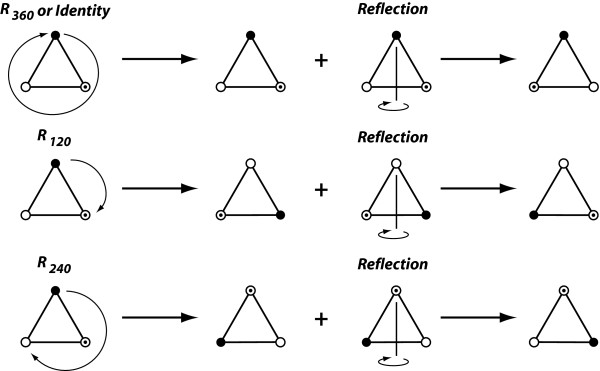
\includegraphics[scale=3]{triangle_symmetries}
	\end{center}
	\caption{The symmetries of an equilateral triangle}
	\label{triangle_sym}
\end{figure}
\end{example}

\begin{example}[$D_4$, Symmetries of a Square]
\begin{figure}[H]
	\begin{center}
		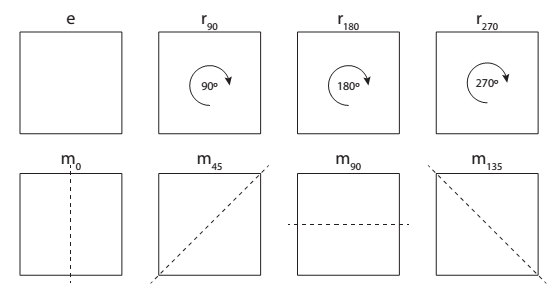
\includegraphics[scale=.75]{square-symmetries}
	\end{center}
	\caption{The symmetries of a square}
	\label{triangle_sym}
\end{figure}

\end{example}

\begin{definition}[Dihedral Group, $D_n$]
In general, $D_n$ is a group with $2n$ elements, where the binary operation is composition. It contains two types of symmetries:
\begin{enumerate}
	\item The rotation $\rho$ is $\frac{2\pi}{n}$ radians clockwise. The set of all rotations is $\langle \rho \rangle = \{1, \rho, \rho^2, \ldots, \rho^{n-1} \}$. 
	\item Let $\e$ be a vertical mirror symmetry. Then the set of all mirror symmetries is $\{\e, \e\rho, \e\rho^2, \ldots, \e \rho^{n-1} \}$. 
\end{enumerate}
\end{definition}


\begin{theorem}[Important Identity for Dihedral Groups]
$\rho \e = \e \rho^{-1}$. 
\end{theorem}
We use this relation to make computations in dihedral groups. 


\begin{theorem}
$\rho^i \e = \e \rho^{-i}$
\end{theorem}
\begin{proof}
By induction, using the above claim. 
\end{proof}

\begin{example}[Uniqueness of rotations/mirror symmetries]
Can two elements in the mirror symmetry set be equal, or equal to an element in the set of rotations? No! Suppose $\e \rho^i = \e \rho^j$. Then $\rho^i = \rho^j$, which implies $i = j$. Now suppose $\e \rho^i = \rho^j$, which implies $\e = \rho^{j-i}$. However this implies $\e$ is a rotation, which is nonsense.
\end{example}

\begin{example}[Mirror Symmetries are a Coset]
Observe that the set of mirror symmetries is simply $\e \langle \rho \rangle$, thus they are a left coset of the cyclic group of rotations.  Then
\begin{equation}
	D_n / \langle \rho \rangle = \{ \langle \rho \rangle, \e \langle \rho \rangle\}
\end{equation}
Since $|D_n| = 2n$ and $|\langle \rho \rangle| = n$, we know that by Lagrange's theorem, $[D_n : \langle \rho \rangle] = 2$. 
\end{example}

\begin{example}
In $D_5$, compute (simplify)
\begin{equation}
\rho \e^7 \rho \e \rho^2 \e \rho^{-3} \e^{-1}
\end{equation}
We know that $\rho \e = \e \rho^{-1}$, $\rho^5 = 1$, and $\e^2 = 1$. Then, with the strategy of pushing $\e$ to the left,
\begin{align*}
	\rho \e^7 \rho \e \rho^2 \e \rho^{-3} \e^{-1} &= \rho \e \rho \e \rho^2 \e \rho^{2} \e \tag{$\rho^{-3} = \rho^{2}, \e^{-1} = \e$} \\
	&= \rho \e \rho \e \rho^2 \e \rho \e \rho^{-1} \\
	&= \rho \e \rho \e \rho^2 \e \e \rho^{-1} \rho^{-1} \\
	&= \rho \e \rho \e \rho^2 \rho^{-1} \rho^{-1} \\
	&= \rho \e \rho \e \\
	&= \rho \e \e \rho^{-1} \\
	&= 1
\end{align*}
\end{example}

\subsection{Quotient Groups}

\begin{definition}[Quotient Group]
Let $G$ be a group and $N \trianglelefteq G$ (that is, $N$ is a normal subgroup of $G$). Let $G/N = \{gN|g \in G\}$ be the set of left cosets of $N$ in $G$. Then the quotient group of $G$ by $N$ is the group $(G/N, \cdot)$, where $\cdot$ is the binary operation on $G/N$ defined for all $g_1 N, g_2 N \in G / N$ by $g_1 N g_2 N = g_1g_2N$. 
\end{definition}

\begin{theorem}
In the above definition, $G/N$ is a group. 
\end{theorem}
\begin{proof}
Binary operation well-defined: We need to check that $\cdot: G/N \times G/N \to G/N$, where $(g_1N, g_2N) \to g_1 g_2 N$ is well-defined (A function is well-defined if it gives the same result when the representation of the input is changed without changing the value of the input. In this context, we show that the definition of multiplication depends on only the cosets and not on the coset representatives). Suppose that $g_1 N = g'_1 N$ and $g_2 N = g'_2 N$, so we want to show $g_1 g_2 N = g'_1 g'_2 N$. Then $g_1N = g'_1 N \iff (g'_1)^{-1} g_1 \in N$ and $g_2 N = g'_2 N \iff (g'_2)^{-1} g_2 \in N$. We then want to show $(g'_1g'_2)^{-1}g_1g_2 \in N$. Then
\begin{align*}
	(g'_1g'_2)^{-1}g_1g_2 &= (g'_2)^{-1} (g'_1)^{-1} g_1 g_2 \\
	&= (g'_2)^{-1} n g_2 \tag{$n = (g'_1)^{-1} g_1 \in N$} \\
	&= (g'_2)^{-1} n g'_2 (g'_2)^{-1} g_2 \\
	&= (g'_2)^{-1} n g'_2 n' \tag{$n' = (g'_2)^{-1} g_2 \in N$}\\
	&= (g'_2)^{-1} g'_2 n'' n' \tag{$N$ is normal}\\
	&= n'' n' \in N
\end{align*}
Therefore the binary operation is indeed well-defined. 

We now check the axioms required to be a group.

\begin{enumerate}
	\item Identity: Observe that
	\begin{equation}
		1 \cdot N = N
	\end{equation}

	\item Inverse: Observe that
	\begin{equation}
		(gN)^{-1} = g^{-1}N
	\end{equation}
	because 
	\begin{equation}
		gNg^{-1}N = gg^{-1} N = N
	\end{equation}

	\item Associativity: Follows clearly from the associativity of $G$. 
	\begin{align*}
		(g_1 N g_2 N)(g_3 N) &= (g_1 g_2 N)(g_3 N) \\
		&= g_1 g_2 g_3 N \\
		&= (g_1 N) (g_2 g_3 N) \\
		&= (g_1 N)(g_2 N g_3 N)
	\end{align*}
\end{enumerate}

Therefore $G/H$ is a group. 
\end{proof}

\begin{example}[Examples of Quotient Groups]
\begin{enumerate}
	\item $\mathbb{R}^{\times} / \mathbb{R}_{> 0} = \{\mathbb{R}_{> 0}, (-1) \cdot \mathbb{R}_{> 0}\} \cong \{\pm 1\}$
	\item $\mathbb{Z} / 12 \mathbb{Z} = \{0 + 12 \mathbb{Z}, 1 + 12 \mathbb{Z}, \ldots, 11 + 12 \mathbb{Z} \} $
	\item $(\mathbb{Z} / 12 \mathbb{Z}) / \{0, 4, 8 \} \cong \mathbb{Z} / 4 \mathbb{Z}$. Thus this quotient group has $4$ elements (we can also see this from Lagrange's theorem). Also observe that this is a cyclic group.
\end{enumerate}
\end{example}

\subsection{Isomorphism Theorems}

\begin{theorem}[The First Isomorphism Theorem]
If $\phi:G\to H$ is a homomorphism of groups, then $G / \ker(\phi) \cong Im \phi$. 
\end{theorem}

\begin{proof}
Define $f: G / \ker(\phi) \to Im \phi$ by $f(a \ker(\phi)) = \phi(a)$. We first show $f$ is indeed well-defined. To that end, pick $a \ker(\phi) = b \ker(\phi)$. Therefore there exists some $k \in \ker(\phi)$ such that $a = bk$. Then
\begin{equation}
	\phi(a) = f(a \ker(\phi)) = f(bk \ker(\phi)) = f(b \ker(\phi)) = \phi(b)
\end{equation}
Therefore $f$ is well-defined. We now show $f$ is an isomorphism. 

\begin{enumerate}
	\item $f$ is a homomorphism: 
	\begin{align*}
		f(a \ker(\phi) b \ker(\phi)) &= f(ab \ker(\phi)) \\
		&=  \phi(ab) \\
		&= \phi(a)\phi(b) \tag{$\phi$ is a homomorphism} \\
		&= f(a \ker(\phi)) f(b \ker(\phi))
	\end{align*}

	\item $f$ is surjective: Let $\phi(a) \in Im \phi$. Then $f(a \ker \phi) = \phi(a)$. 
	\item $f$ is injective:  
	\begin{align*}
		\ker(f) &= \{a \ker \phi : f(a \ker \phi) = 1_H \} \\
		&= \{a \ker \phi : \phi(a) = 1_H \} \\
		&= \{\ker \phi \} 
	\end{align*}
	Thus the kernel of $f$ is trivial (the trivial left coset), so $f$ is injective. 
\end{enumerate}

Therefore $f$ is an isomorphism.
\end{proof}

Intuition for this theorem:
\begin{itemize}
	\item This is a more general version of the rank-nullity theorem.
	\item Given vector spaces $V, W$ and a linear transformation $A : V \to W$, this theorem says
	\begin{equation}
		dim( V / \ker A ) = dim (range(A))
	\end{equation}
	or that
	\begin{equation}
		dim(V) - nullity(A) = rank(A)
	\end{equation}
\end{itemize}

\begin{example}[Examples of applications of first isomorphism theorem] Consider the following examples
\begin{enumerate}
	\item $sgn : \R^{\times} \to \{\pm 1 \}$. This is indeed a homomorphism. By the theorem, we know that
	\begin{equation}
		\R^{\times} /\ker(sgn) \cong \{ \pm 1\}
	\end{equation}
	Then $\ker(sgn) = \R_{>0}$. This matches the previous example. 
	\item $\det : GL_2(\mathbb{R}) \to \R^{\times}$. The theorem implies
	\begin{equation}
		GL_2(\mathbb{R}) / \{A \in GL_2(\mathbb{R}) | \det(A) = 1 \} \cong \R^{\times}
	\end{equation}
\end{enumerate}

\end{example}

\begin{theorem}[The Second or Diamond Isomorphism Theorem]
Let $H \leq G$ and $K \trianglelefteq G$. Then $HK / K \cong H / H \cap K$. 
\end{theorem}

\begin{proof}
Define $f : HK / K \to H / H \cap K$ by 
\begin{equation}
	f(hk K) = h (H \cap K)
\end{equation}
We'll first show $f$ is well-defined. Fix $hk, h'k' \in HK$ such that $hk K = h'k'K \in HK/K$. There $h = h'\tilde{k}$ for some $\tilde{k} \in K$. Then
\begin{equation}
	h (H \cap k) = f(hk K) = f(h' \tilde{k} K) = h' (H \cap K)
\end{equation}
Therefore $f$ is well-defined, and we now show $f$ is an isomorphism.
\begin{enumerate}
	\item $f$ is a homomorphism:
	\begin{align*}
	f(h_1 k_1 K \cdot h_2 k_2 K) &= f(h_1 K \cdot h_2 K) \\
	&= f(h_1h_2 K) \\
	&= h_1h_2 (H \cap K) \\
	&= h_1 (H \cap K) h_2 (H \cap K) \\
	&= f(h_1 k_1 K) f(h_2 k_2 K)
	\end{align*}
	\item $f$ is surjective: Clear by the definition of $f$. 
	\item $f$ is injective: We'll show the kernel of $f$ is trivial (in this context, the trivial left coset). 
	\begin{align*}
		\ker(f) &= \{ hk \cdot K | f(hk \cdot K) = H \cap K \} \\
		&= \{ hk \cdot K | h (H \cap K) = H \cap K \} \\
		&= \{ hk \cdot K | h \in H \cap K \} \tag{$h (H\cap K) = H \cap K \iff h \in H\cap K$} \\
		&= \{K \}
	\end{align*}
\end{enumerate}
\end{proof}

\subsection{Actions, Orbits, and Stabilizers}
\begin{definition}[Action]
An action of a group $G$ on $X$ (or we say $G$ acts on $X$) is a function $G \times X \to X$, $(g,x) \to gx$ where
\begin{enumerate}
	\item $1_G x = x \quad \forall x \in X$ 
	\item $g(hx) = (gh)x \quad \forall g,h \in G, \forall x \in X$
\end{enumerate}
\end{definition}

\begin{example}[Group Actions]
\begin{enumerate}
	\item Set: $\R^n$, Group: $GL_n(\R)$, Action: $(A,v) \to Av$. In $\R^2$, we can see that
	\begin{equation}
		\begin{pmatrix}
		a & b \\
		c & d
		\end{pmatrix}
		\begin{pmatrix}
		v_1 \\ v_2
		\end{pmatrix}
		=
		\begin{pmatrix}
		av_1 + bv_2 \\
		cv_1 + dv_2 
		\end{pmatrix}
		\in \R^2
	\end{equation}
	Observe that the two axioms required to be an axiom are satisfied, since the identity matrix preserves vectors and matrix/vector multiplication is associative. 
	\item Set: $\{1, \ldots, n\}$, Group: $S_n$, Action: $(\sigma, i) \to \sigma(i)$. Observe that the two axioms are satisfied. The identity permutation fixes an index and the composition of permutations is associative. 
	\item Set: $G$, Group: $G$, Action: $(g,h) \to gh$. The identity element of $G$ maps $1_G h = h$ and since $G$ is a group, multiplication is associative. 
	\item Set: $G$, Group: $G$, Action: $(g,x) \to gxg^{-1}$. Let's verify the axioms:
	\begin{enumerate}
		\item Suppose $g=1$. Then $(1,x) \to 1 x 1^{-1} = x$. 
		\item Observe that
		\begin{equation}
			g(h(x)) = g(hxh^{-1}) = g(hxh^{-1})g^{-1} 
		\end{equation}
		and
		\begin{equation}
			(gh)(x) = gh x (gh)^{-1} = gh x h^{-1} g^{-1}
		\end{equation}
	\end{enumerate}
	\item Set: Set of all subgroups of $G$, Group: $G$, Action: $(g,H) \to gHg^{-1}$. We need to show that $gHG^{-1}$ is a subgroup if $H$ is a subgroup (this shows that $G \times (subgroup) \to (subgroup))$. Let's verify the axioms required to be a subgroup:
	\begin{enumerate}
		\item Identity: Note that $1 \in H$ since $H \leq G$. Thus $g1g^{-1} = 1\in gHg^{-1}$. 
		\item Closed under products: Let $ghg^{-1}, gh'g^{-1} \in gHg^{-1}$. Then
		\begin{align*}
			(ghg^{-1})(gh'g^{-1}) &= ghh'g^{-1} \\
			&= g\tilde{h} g^{-1} \in gHg^{-1} \tag{$H$ closed under multiplication}
		\end{align*}
		\item Closed under inverses: Note that $(ghg^{-1})^{-1} = gh^{-1}g^{-1} \in H$ since $H$ is closed under inverses. 
	\end{enumerate}
	Therefore $gHg^{-1}$ is a subgroup. Now, let's verify the axioms to should this is indeed an action [[?]]:
	\begin{enumerate}
		\item $1 gHg^{-1}= gHg^{-1}$
		\item ??
	\end{enumerate}
	\item Set: Pairs of distinct elements from $\{1, \ldots, n\}$, Group: $S_n$, Action: $\sigma(i,j) = (\sigma(i), \sigma(j))$. 
\end{enumerate}
\end{example}

\begin{definition}[Orbit]
Given $x \in X$ the orbit of $x$ is 
\begin{equation}
	O(x) = O_x = \{gx | g \in G\}
\end{equation}
This is the set of all elements that can be reached from $x$ by applying elements from $G$. 
\end{definition}

\begin{example}[Examples of Orbits]
\begin{enumerate}
	\item Let $X = \{1, \ldots, n\}$. Suppose $G = S_n$. Then the orbit of each element is the whole set, $X$. 
	\item $H$ is normal if and only if all if its orbits only contain one element [[?]]. 
\end{enumerate}
\end{example}

\begin{definition}[Stabilizer, Isotropy Subgroup]
Let $X$ be a $G$-set and $x \in X$. The stabilizer of $x$ is 
\begin{equation}
	G_x = Stab_G(x) = \{ g\in G | gx = x \}
\end{equation}
also called the isotropy subgroup of $x$. 
\end{definition}

\begin{theorem}[The stabilizer of a group element is a subgroup]
$G_x \leq G$
\end{theorem}
\begin{proof}
We verify the three axioms required to be a subgroup:
\begin{enumerate}
	\item Identity: Note that $1 x = x$, therefore $1 \in G_x$. 
	\item Closed under products: Let $a,b \in G_x$. We need to show that $ab \in G_x$, or that $(ab)x = x$. Then,
	\begin{equation}
		(ab)x = a(bx)= ax = x
	\end{equation}
	\item Closed under inverses: Let $a \in G_x$. We know $ax = x$. Therefore, applying $a^{-1}$ on the left, we get that
	$a^{-1} a x = a^{-1} x$. This simplifies to $x = a^{-1} x$. Thus $a^{-1} \in G_x$. 
\end{enumerate}
Thus $G_x$ is a subgroup. 
\end{proof}

\begin{theorem}[Orbit-Stabilizer Theorem]
There is a bijection 
\begin{equation}
	f : G / G_x \to O_x
\end{equation}
In words, there is a bijection between the collection of all cosets of the stabilizer and the orbit. In particular, 
\begin{equation}
	[G:G_x] = |O_x|
\end{equation}
(Recall we defined $|G / G_x|$ to be $[G:G_x]$). 
\end{theorem}
\begin{proof}
Define 
\begin{equation}
	f : G / G_x \to O_x 
\end{equation}
by
\begin{equation}
	f(gG_x) = gx
\end{equation}
We will first verify that $f$ is well-defined. In this context, this means that the output of the function does not depend on what representative from the left coset is chosen. To that end, suppose $gG_x = hG_x$. We need to show that $gx = hx$. Equivalently, we need to show that $h^{-1}gx=x$, or that $h^{-1}g \in G_x$ (the stabilizer of $x$). However, this last characterization follows directly from the assumption that 
\begin{equation}
	gG_x = hG_x
\end{equation}

We now show that $f$ is surjective. This is clear from the definition of the function. To get an element $gx$, we simply need to input $g$.

We now show that $f$ is injective (note here that $f$ is not a homomorphism. Thus we cannot use the trick that $f$ is injective if and only if its kernel is trivial). Suppose that $f(gG_x) = f(hG_x)$. Hence, $gx = hx$, so $h^{-1}gx = x$. Therefore, $h^{-1}g \in G_x$, which implies that $gG_x = hG_x$. 
\end{proof}

\begin{example}[Examples of Orbit-Stabilizer Theorem]
\begin{enumerate}
	\item Suppose $D_3$ acts on the vertices of a triangle. That is, $G=D_3$ and $X=\{a,b,c\}$. Observe that $O_a = \{a,b,c\}$, because a rotation allows us to reach any other vertex starting from $a$. Next, $G_a = \{1, \text{ reflection at } a\}$. Observe that 
	\begin{equation}
		[G:G_a] = \frac{|G|}{|G_a|} = \frac{6}{2} = 3
	\end{equation}
	and
	\begin{equation}
		|O_a| = 3
	\end{equation}
	Therefore the theorem holds.

	\item Suppose $S_5$ acts on $\{1,2,3,4,5\}$. Then 
	\begin{equation}
		G_5 \cong S_4
	\end{equation}
	In words, the stabilizer of $5$ is simply the set of permutations that keep $5$ fixed, which is equivalent to the set of permutations of $\{1,2,3,4\}$. Note that $O_5 = \{1,2,3,4,5\}$. And
	\begin{equation}
		[G:G_5] = \frac{|S_5|}{|G_5|} = \frac{120}{24} = 5	
	\end{equation}
	and
	\begin{equation}
		|O_5| = 5
	\end{equation}
	Therefore the theorem holds.
\end{enumerate}
\end{example}

\begin{definition}[Transitive action]
	We say that an action of $G$ on $X$ is transitive if for every $x,y \in X$, there is an element $g \in G$ such that $gx = y$. In words, this means that we can arrive at $y$ from $x$ by applying an element from $G$. 
\end{definition}

\begin{example}[Transitive actions]
\begin{enumerate}
	\item The action of $S_5$ on $\{1,2,3,4,5\}$ is transitive. 
	\item The action of $GL_n(\R)$ on $\R^n$ is not transitive. Consider the zero vector. Then any matrix we apply to the zero vector will still give us the zero vector. Thus, we cannot reach another vector in $\R^n$. 
	\item The multiplication action of $G$ on itself is transitive. To get to y from $x$, we can apply $g=yx^{-1}$.  
\end{enumerate}
\end{example}

\begin{definition}[Action induces equivalence relation]
	The action of any group $G$ on $X$ induces an equivalence relation by saying $x \sim y$ if there exists a $g \in G$ such that $gx = y$. 
\end{definition}
\begin{proof}
We'll show that this is indeed an equivalence relation. We need to verify three axioms:
\begin{enumerate}
	\item Reflexive: We want to show that $x\sim x$. Let $g = 1$. Then $1 \cdot x = x$.
	\item Symmetric: Suppose $x \sim y$. We want to show that $y \sim x$. Since $x \sim y$, there exists a $g \in G$ such that $gx = y$. This implies $x = g^{-1}y$. Therefore $y \sim x$. 
	\item Transitive: Suppose $x\sim y$ and $y \sim z$. We want to show that $x \sim z$. By definition, there exist $g,h \in G$ such that $gx = y$ and $hy = z$. Thus $hgx = z$. Since the binary operation of $G$ is closed, we know $gh \in G$, so that $x \sim z$. 
\end{enumerate}
\end{proof}

\begin{remark}
The equivalence class of $x \in X$ is the orbit of $x$, $O_x$. 
\end{remark}

\begin{theorem}
An action is transitive if and only if there exists an $x \in X$ such that $O_x = X$. That is, all elements of $X$ have the same equivalence class. 
\end{theorem}
\begin{proof}
	\color{Red}{TODO}
\end{proof}

\begin{definition}[Conjugation action, conjugacy classes, conjugate]
	Consider the action of $G$ on itself by $g(x) = gxg^{-1}$. We call this the conjugation action. The equivalence classes created by this action are called the conjugacy classes of $G$. We say that two elements in $x,y\in G$ are conjugate if they belong to the same conjugacy class. 
\end{definition}

\begin{example}
	In $S_5$, the elements $(1 2)(3 4)$ and $(5 2)(1 3)$ are conjugate. In other words, there exists a $\sigma \in S_5$ such that
	\begin{equation}
		\sigma (1 2)(3 4) \sigma^{-1} = (5 2)(1 3)
	\end{equation}
	One $\sigma$ that works is
	\begin{equation}
		\sigma(1)=5, \quad \sigma(2)=2, \quad \sigma(3)=1, \quad \sigma(4)=3, \quad \sigma(5)=4
	\end{equation}
	We can generate this $\sigma$ by recalling that
	\begin{align*}
	\sigma (1 2)(3 4) \sigma^{-1} &= \sigma (1 2) \sigma^{-1} \sigma (3 4) \sigma^{-1} \\
	&= (\sigma(1) \sigma(2))(\sigma(3) \sigma(4))
	\end{align*}
	Thus we want to choose a $\sigma$ such that these two cycles are equivalent to the two given cycles. 
\end{example}

\begin{definition}[Fixed points]
	For any element $g\in G$, let $X^g = \{x\in X|gx = x\}$. In words, this is the set of all elements in $X$ such that $g$ acts on them like the identity. 
\end{definition}

\begin{example}[Fixed points]
\begin{enumerate}
	\item Let $G = D_3$ and $X = \{a,b,c\}$ be the vertices of a triangle. Then $X^\rho = \emptyset$. However, the set of fixed points of the reflection through $c$ is simply $\{c\}$. 
	\item Let $G = GL_2(\R)$ and $X = \R^2$. Then
	\begin{align*}
	X^{\begin{pmatrix}
	0 & 1 \\
	1 & 0
	\end{pmatrix}}
	&= \left\{ \begin{pmatrix} a \\ b \end{pmatrix}\in \R^2 \vert \begin{pmatrix}
	0 & 1 \\
	1 & 0
	\end{pmatrix} \begin{pmatrix} a \\ b \end{pmatrix} = \begin{pmatrix} a \\ b \end{pmatrix}\right\} \\
	&=  \left\{ \begin{pmatrix} a \\ b \end{pmatrix}\in \R^2 \vert \begin{pmatrix}b \\ a \end{pmatrix} = \begin{pmatrix} a \\ b \end{pmatrix}\right\} \tag{where the first and second coord are the same}\\
	&= span\left\{ \begin{pmatrix}
	1 \\ 1
	\end{pmatrix} \right\} 
	\end{align*}
\end{enumerate}
\end{example}

\begin{theorem}[Burnside]
Let $G$ act on $X$. Suppose that $G,X$ are finite. Then, 
\begin{equation}
	N = \text{ \# of orbits (equivalence classes) } = \frac{1}{|G|} \sum_{g\in G} |X^g|
\end{equation}
\end{theorem}
\begin{proof}
	Let's count 
	\begin{equation}
		|\{(g,x): gx = x \}|
	\end{equation}
	in two ways.
	\begin{enumerate}
		\item By counting "over $G$" (i.e.\ how many elements each $g$ contributes): For each $g$, this simply the number of points $g$ fixes
		\begin{equation}
			\sum_{g \in G} |X^g|
		\end{equation}
		\item By counting "over $X$": For each $x$, this is how many elements $g \in G$ that fix $x$:
		\begin{equation}
			\sum_{x\in X} |G_x|
		\end{equation}
		By the orbit-stabilizer theorem, we know that 
		\begin{equation}
			\frac{|G|}{|G_x|} = |O_x|
		\end{equation}
		Therefore
		\begin{align*}
		\sum_{x\in X} |G_x| &= \sum_{x\in X} \frac{|G|}{|O_x|} \\
		&= |G| \sum_{x\in X} \frac{1}{|O_x|} \\
		&= |G| \sum_{\text{orbits}} \sum_{\text{elements}} \frac{1}{|O_x|} \\
		&= |G| \sum_{\text{orbits}} 1 \\
		&= |G| N
		\end{align*}
	\end{enumerate}
	Equating these two ways of counting the number of elements in the set proves the theorem. 
\end{proof}

\begin{exercise}
In how many ways can one color the vertices of a square using $10$ distinct colors? Or, how many orbits are there for the action of $D_4$ on the set of colorings of the vertices of a square using the colors. 
\end{exercise}
\begin{solution}
	We can use Burnside's theorem to complete this calculation.
	\begin{center}
	\begin{tabular}{c|l}
	Element $g \in G$ & $|X^g|$ \\
	\hline 
	$1$ & $10^4 = 10000$ \\
	$\rho$ & $10$ (all vertices share same color) \\
	$\rho^2$ & $10^2 = 100$ (opposite vertices share same color) \\
	$\rho^3$ & $10$ (same as $\rho$)\\
	Edge Reflection (x2) & $10^2 = 100$ (adjacent vertices across reflection line same) \\
	Vertex Reflection (x2) & $10^3 = 1000$ (vertices not on reflection line same)
	\end{tabular}
	\end{center}
	Then by Burnside's Theorem, we know that
	\begin{equation}
		N = \frac{1}{8}(10,000 + 10 + 100 + 10 + 2 \times 100 + 2 \times 1000)
	\end{equation}
\end{solution}

\begin{definition}[Free, faithful action]
	Let $G$ be a group that acts on a set $X$. 
	\begin{enumerate}
		\item The action is said to be faithful if for all $x \in X$
		\begin{equation}
			gx = x \implies g = 1
		\end{equation}
		Thus the only element that acts like the identity is actually the identity $g=1$. Alternatively, 
		\begin{equation}
			\cap_{x \in X} G_x = \{1\}
		\end{equation}
		\item The action is free if for all $g\in G$ and for all $x \in X$
		\begin{equation}
			gx = x \implies g = 1
		\end{equation}
		Alternatively, this means all stabilizers are trivial. We have that for all $x \in X$, 
		\begin{equation}
			G_x = \{1\}
		\end{equation}
		 Or, any element which has a fixed point is the identity element. 
	\end{enumerate}
\end{definition}

Observations:
\begin{itemize}
	\item If free, then faithful.
\end{itemize}

\begin{example}[Free, faithful actions]
\begin{enumerate}
	\item The action of $G$ on itself by left multiplication is free. 
	\item The action of $D_n$ on the vertices of an $n$-gon is faithful but not free.
	\item Suppose $GL_2 (\R)$ acts on $\R^2$. This action is not free, but it is faithful. It's not free because 
	the zero vector is always mapped back to the zero vector. It is faithful since $Av = v$ implies $A$ is the identity matrix (to see this, consider $v = \begin{pmatrix} 1 \\ 0\end{pmatrix}$ and $v = \begin{pmatrix} 0 \\ 1\end{pmatrix}$).
\end{enumerate}
\end{example}

\subsection{Multiplicative group of integers modulo n}

\begin{definition}[Coprime]
	An integer $a$ is coprime to $n$ if the only positive divisor of both $a$ and $n$ is 1.
\end{definition}

\begin{definition}[$(\mathbb{Z}/n \mathbb{Z})^{\times}$]
\begin{equation}
	(\mathbb{Z}/n \mathbb{Z})^{\times} = \{1 \leq a \leq n - 1 | a \text{ coprime to } n\}
\end{equation}
$n \geq 2$. This is called the multiplicative group of integers modulo $n$, where the binary operation is multiplication and taking the remainder upon dividing by $n$. 
\end{definition}

\begin{example}[$(\mathbb{Z}/n \mathbb{Z})^{\times}$]

\begin{center}
\begin{tabular}{c|c}
$n$ & ($(\mathbb{Z}/n \mathbb{Z})^{\times}$) \\
\hline 
2 & \{ 1 \} \\
3 & \{1 , 2\} \\
4 & \{1, 3\} \\
5 & \{1, 2, 3, 4\} \\
6 & \{1, 5\}
\end{tabular}
\end{center}
\end{example}

\begin{example}[Computations in $(\mathbb{Z}/n \mathbb{Z})^{\times}$]
Suppose $n=5$. Then we consider $(\mathbb{Z}/5 \mathbb{Z})^{\times}$. 
\begin{enumerate}
	\item $1 \cdot 2 = 2$ 
	\item $2 \cdot 3 = 1$
	\item $2 \cdot 2 = 4$
	\item $3 \cdot 3 = 4$
\end{enumerate}
\end{example}

\begin{theorem}
$(\mathbb{Z}/n \mathbb{Z})^{\times}$ is a group.
\end{theorem}
\begin{proof}
We verify the axioms:
\begin{enumerate}
	\item Unit: The unit element is $1$, since $1$ is coprime to every number and acts an identity under multiplication.
	\item Inverse: Define a function for a fixed $g \in (\mathbb{Z}/n \mathbb{Z})^{\times}$ by $f : (\mathbb{Z}/n \mathbb{Z})^{\times} \to (\mathbb{Z}/n \mathbb{Z})^{\times}$ where $f(x) = gx$. To show that $g$ has an inverse, it suffices to show that $f$ is surjective. If $f$ is surjective, then there must exist some $x \in (\mathbb{Z}/n \mathbb{Z})^{\times}$ such that $gx = 1$. However, since $(\mathbb{Z}/n \mathbb{Z})^{\times}$ is finite, it is enough to show that $g$ is injective (so that $f$ must also be surjective.) suppose that $gx = gy$ for some $x,y \in (\mathbb{Z}/n \mathbb{Z})^{\times}$. Then, for some $\alpha, \beta \in \mathbb{Z}$
	\begin{equation}
		gx - n\alpha = gy - n\beta \tag{equality of integers}
	\end{equation}
	this implies
	\begin{equation}
		g(x-y) = n(\alpha - \beta)
	\end{equation}
	so that $n$ divides $g(x-y)$. Next, recall that $n$ is coprime to $g$ (by the definition of the set/group), so  $n | (x-y)$. However, since $x,y \in (\mathbb{Z}/n \mathbb{Z})^{\times}$, the difference in absolute value of $x$ and $y$ must be less than $n$. This implies that $x=y$, which proves injectivity.
\end{enumerate}
\end{proof}

\begin{theorem}[Fermat's Little Theorem]
	For a prime number $p$ and $1 \leq x \leq p-1$, we have $x^{p-1} - 1$ is divisible by $p$.
\end{theorem}
\begin{proof}
	Note that $x \in (\mathbb{Z}/p \mathbb{Z})^{\times}$ (since $p$ is prime and $x$ is less than $p$). Let $k$ be the order of $x$ and consider 
	\begin{equation}
		\langle x \rangle = \{1,x,x^2,\ldots,x^{k-1}\}
	\end{equation}
	by Lagrange's theorem, $|\langle x \rangle|$ divides $|(\mathbb{Z}/n \mathbb{Z})^{\times}|$. Thus $k$ divides $p-1$ (because $|\langle x \rangle|$ is $k$ and$|(\mathbb{Z}/n \mathbb{Z})^{\times}|$ is $p-1$, since $p$ is prime). Then there exists some $t$ such that $p-1 = k \cdot t$. Thus
	\begin{equation}
		x^{p-1} = x^{k\cdot t} = (x^k)^t = 1^t = 1 \tag{mod $p$}
	\end{equation}
\end{proof}

\begin{theorem}
	Let $p \neq q$ be odd primes. Then
	\begin{equation}
		(\mathbb{Z}/pq \mathbb{Z})^{\times} \cong (\mathbb{Z}/p \mathbb{Z})^{\times} \times (\mathbb{Z}/q \mathbb{Z})^{\times}
	\end{equation}
\end{theorem}
\begin{proof}
	Define a homomorphism $\phi: (\mathbb{Z}/pq \mathbb{Z})^{\times} \cong (\mathbb{Z}/p \mathbb{Z})^{\times} \times (\mathbb{Z}/q \mathbb{Z})^{\times}$ by taking remainders for division by $p$ and $q$ separately. 
	\begin{example}
	Suppose $p=3$ and $q=5$. Then $\phi(11) = (2, 1)$.
	\end{example}
	It suffices to check that $\phi: (\mathbb{Z}/pq \mathbb{Z})^{\times} \cong (\mathbb{Z}/p \mathbb{Z})^{\times}$ is a homomorphism. This requires checking that $ab$ reduces mod $p$ to the product of the reductions of $a$ and $b$. 
	\begin{example}$p = 3$ and $q = 5$.
	\begin{equation}
	7 \cdot 11 = 77 = 2
	\end{equation}
	and 
	\begin{equation}
	1 \cdot 2 = 2
	\end{equation}
	\end{example}
	Next we'll show $\phi$ is injective. We'll show that $\ker \phi$ is trivial.
	\begin{align*}
		\ker \phi &= \{1 \leq a \leq pq - 1 | \phi(a) = (1,1)\} \\
		&= \{1 \leq a \leq pq - 1 \Big\vert p | (a-1), q | (a-1) \} \\ 
		&= \{1 \leq a \leq pq - 1 \Big\vert pq | (a-1) \} \\
		&= \{1\}
	\end{align*}
	To show surjectivity, we'll show that the domain and the range have the same size (we can do this since we've already shown $\phi$ is injective.) Then
	\begin{equation}
		|(\mathbb{Z}/pq \mathbb{Z})^{\times}| = (p-1)(q-1) 
	\end{equation}
	and
	\begin{equation}
		|(\mathbb{Z}/pq \mathbb{Z})^{\times}| = pq - q - p + 1
	\end{equation}
	because there are $pq$ total possible elements, but $q$ are divisible by $p$, $p$ divisible by $q$, and 1 element ($pq$) that is divisible by both $p$ and $q$. 
\end{proof}

\begin{definition}[Permutation representation of action]
	Let $G$ be a group that acts on $\{1,\ldots, n\}$. Associated to the action is a homomorphism $\lambda : G \to S_n$, defined by 
	\begin{equation}
		\lambda(g)(i) = gi
	\end{equation}
	where the RHS is the action of $g$ on $i$, $i \in \{1,\ldots, n\}$.
\end{definition}
We need to confirm that $\lambda$ is indeed a homomorphism.
\begin{proof}
\begin{align*}
	\lambda(gh)(i) &= gh(i) \\
	&= g(h(i)) \tag{since action} \\
	&= \lambda(g)(h(i)) \tag{definition of $\lambda$} \\
	&= \lambda(g)(\lambda (h)(i)) \tag{definition of $\lambda$} 
\end{align*}
\end{proof}

For completeness, we should also check $\lambda(g)$ is indeed a permutation for every $g \in G$.
\begin{proof}
Incomplete (some weird proof with the inverse?)
\end{proof}

\begin{theorem}
If $\lambda : G \to S_n$ is a homomorphism, we can define an action of $G$ on $\{1,\ldots, n\}$ by
\begin{equation}
	g(i) = \lambda(g)(i)
\end{equation}
\end{theorem}
\begin{proof}
We check the two conditions required to be an action:
\begin{enumerate}
	\item $1(i) = \lambda(1)(i) = id (i) = i$
	\item $gh(i) = \lambda (gh)(i) = \lambda(g)(\lambda (h)(i)) = \lambda(g)(h(i)) = g(h(i))$
\end{enumerate}
\end{proof}

\begin{example}
	Let $D_4$ action of the vertices of a square. We can enumerate the values of the homomorphism $\lambda : D_4 \to  S_4$.
	\begin{enumerate}
		\item $\lambda(id) = id$
		\item $\lambda(\rho) = (1 2 3 4)$
		\item $\lambda(\rho^2) = (13)(24)$ 
		\item $\lambda(\rho^3) = (1 4 3 2)$
		\item $\lambda(\e) = (1 2)(34)$
		\item and so on
	\end{enumerate}
\end{example}

\begin{theorem}
Under the above assumptions: $\lambda$ is injective if and only if the action of $G$ on $X$ (which we can think of as $\{1,\ldots, n\}$) is faithful.
\end{theorem}
\begin{proof}
	Since $\lambda$ is a homomorphism, we can prove it is injective by showing its kernel is trivial. Then
	\begin{equation}
		\ker \lambda = \{g\in G | \lambda(g)(i) = i \quad \forall i \in X\}
	\end{equation}
	Hence, $\ker \lambda = \{1\}$ if and only if the action is faithful.
\end{proof}

\begin{theorem}[Cayley]
	Let $G$ be a group of order $n$. Then, there exists an injective homomorphism $\phi : G \to S_n$.
\end{theorem}
\begin{proof}
	Consider the action of $G$ on itself by (left) multiplication. Associated to this action is a homomorphism $\phi : G \to S_n$. This action is free (shown in homework), and therefore faithful, so $\phi$ is injective by the above claim.
\end{proof}

\begin{example}
	Take $G = \mathbb{Z} / 3 \mathbb{Z} = \{1,2,3\}$ (where $3 = 0$). Then $\phi : G \to S_3$ has elements
	\begin{enumerate}
		\item $\phi(3) = id$
		\item $\phi(2) = (1 3 2)$ (since $1 + 2 = 3$ and $3 + 2 = 5 = 2$ and $2 + 2 = 4 = 1$)
		\item $\phi(1) = (1 2 3)$
	\end{enumerate}
\end{example}

\begin{theorem}
	If $|G| = n$, then $G$ is isomorphic to a subgroup of $S_n$. Indeed $\phi : G \to Im(\phi) \subset S_n$.
\end{theorem}

\subsection{p-Groups}

\begin{definition}[$p$-Group]
	Let $p$ be a prime number. $G$ is a $p$-group if $|G|$ is a power of $p$. 
\end{definition}

\begin{theorem}[Cardinality of set of fixed points of action of set on $p$-group equals cardinality of set mod $p$]\label{lemma:favlemma}
	Let $G$ be a $p$-group that acts on a finite set $X$. Let $X^G = \cap_{g \in G} X^g$ where $X^g = \{x\in X| gx =x\}$, that is those $x\in X$ such that for all $g\in G$, $gx = x$. Then $p$ divides $|X| - |X^G|$, that is
	\begin{equation}
		|X^G| \equiv |X| \quad (mod p)
	\end{equation}
\end{theorem}
\begin{proof}
Let $x_1, \ldots, x_m$ be the representatives for the orbits of $G$ on $X$ (recall that the the disjoint union of orbits of these representatives cover $X$). Let's partition these elements into those in $X^G$ and those not. Thus suppose that $x_1, \ldots, x_k \in X^G$ and $x_{k+1}, \ldots, x_m \not\in X^G$. Then
\begin{equation}
	|X| = \sum_{i=1}^m |O(x_i)| = \sum_{i=1}^k |O(x_i)| \sum_{j=k+1}^m |O(x_j)|
\end{equation}
Then
\begin{equation}
	\sum_{i=1}^k |O(x_i)| = |X^G|
\end{equation}
and by the orbit-stabilizer theorem
\begin{equation}
	\sum_{j=k+1}^m |O(x_j)| = \sum_{j=k+1}^m \frac{|G|}{|G_{x_j}|}
\end{equation}
Notice that $|G|$ is divisible by $p$. Further, $|G_{x_j}|$ must be divisible by $p$ since it is a subgroup of $G$ (this follows from Lagrange's theorem). Therefore, $|X|$ equals $|X^G|$ plus the sum of things divisible by $p$, so that we must have that $p$ divides $|X| - |X^G|$. 
\end{proof}

\begin{theorem}[A $p$-group has a non-trivial center]
	Let $G$ be a $p$-group. Then $Z(G) \neq \{1\}$.  In words, there has to be a non-trivial element of the group that commutes with everything else.
\end{theorem}
\begin{proof}
	Let $X = G$ and consider the action of $G$ on $X$ by conjugation. By the above theorem, we know that $p$ divides $|X| - |X^G|$. Therefore since $p$ divides $|X|$, we must have that $p$ divides $|X^G|$. Now
	\begin{align*}
		X^G &= \{x\in X | \forall g \in G, g(x) = x\} \\
		&= \{x\in X | \forall g \in G, gxg^{-1} = x\} \\
		&= \{x\in X | \forall g \in G, gx = xg\} = Z(G)
	\end{align*}
	We always have that $1 \in Z(G)$. Now since $p$ divides $|X^G|$, we must have that $Z(G) \neq \{1\}$, since no prime $p$ divides 1.  
\end{proof}

\begin{corollary}
	Let $p$ be a prime number and let $G$ be a group of order $p^2$. Then $G$ is abelian.
\end{corollary}
\begin{proof}	
	Consider $Z(G)$. By Lagrange's theorem, we must have that $|Z(G)| = p, p^2$ (the above theorem rules out $1$. The only other possible divisors are $p$ and $p^2$ since $p$ is prime). There are two cases to consider.
	\begin{enumerate}
		\item Case 1: $|Z(G)| = p^2$. Then $Z(G) = G$. Thus since $Z(G)$ is abelian, $G$ is abelian.
		\item Case 2: $|Z(G)| = p$. Then by Lagrange's theorem, $| G / Z(G) | = p$ $G / Z(G)$ is cyclic (since $Z(G)$ is normal), Thus $G$ is abelian.
	\end{enumerate}
\end{proof}

This same result need not hold for higher powers of $p$. For example, consider $D_8$. $2^3 = 8$. But $|D_8|$ is not abelian. 

\begin{theorem}[Cauchy]
	Let $G$ be a finite group and suppose that $p \big\vert |G|$ for some prime $p$. Then there exists an element of order $p$ in $G$. 
\end{theorem}

\begin{proof}
	Let's start by proving the simple case of $p=2$. Therefore $|G|$ is even. We can pair each element in $G$ with its inverse. Note that $1 = 1^{-1}$ so the identity element is paired with itself. Since $|G|$ is even, there must exist $1 \neq g \in G$ such that $g = g^{-1}$. Then $g^2 = 1$. Thus there exists an element of order $2$. 

	Let's now prove the general case. Define the set $X$ as 
	\begin{equation}
		X = \{(g_1, \ldots, g_p) | g_1g_2 \cdots g_p = 1, \quad g_1, g_2, \ldots, g_p \in G\}
	\end{equation}
	Then $\Z / p \Z$ acts on $X$ by $a(g_1, \ldots, g_p)$ by cyclic rotation of $a$ times of $(g_1, \ldots, g_p)$ where $a \in \{0,1,\ldots, p-1\}$. 
\end{proof}

\begin{example}[Example of Cauchy's Theorem]
	Consider $G = S_5$. If $p=3$, then $(123)$ is an example of an element with order $3$. If $p=5$, then $(12345)$ is an example of an element with order $5$. 
\end{example}

\subsubsection*{Summary of $p$-Groups}
\begin{enumerate}
	\item Any group of order $p$ is cyclic.
\end{enumerate}

\begin{theorem}[Correspondence Theorem]
	Let $G, H$ be groups, and let $\phi : G \to H$ be a group homomorphism. Then there exists a correspondence (i.e.\ a bijection)
	\begin{equation*}
		\{\text{Subgroups $K$ of $G$ containing $\ker \phi$}\} \iff \{\text{Subgroups $L$ of $H$ contained in $Im(\phi)$}\}
	\end{equation*}
	given by $K \mapsto \phi(K)$ and $L \mapsto \phi^{-1}(L)$. In addition, let $K_1$ and $K_2$ be subgroups of $G$ containing $\ker(\phi)$ and $L_1$ and $L_2$ subgroups $L$ of $H$ contained in $Im(\phi)$. 
	\begin{enumerate}
		\item $K_1 \leq K_2 \implies \phi(K_1) \leq \phi(K_2)$
		\item $L_1 \leq L_2 \implies \phi^{-1}(L_1) \leq \phi^{-1}(L_2)$
	\end{enumerate}
	and
	\begin{enumerate}
		\item $K_1 \leq K_2 \implies [K_2 : K_1] = [\phi(K_2) : \phi(K_1)]$
		\item $L_1 \leq L_2 \implies [L_2 : L_1] = [\phi(L_2) : \phi(L_1)]$
	\end{enumerate}
\end{theorem}

\begin{theorem}[Sylow's Theorem]
	Let $p$ be a prime number, let $G$ be a finite group, and let $p^n$ be the largest power of $p$ that divides $
	|G|$. Then $G$ contains a subgroup $P$ of order $p^n$. $P$ is called a $p$-Sylow subgroup of $G$. 
\end{theorem}
\begin{proof}

\end{proof}

\begin{theorem}[$p$-Sylow subgroups are conjugate]
	Let $G$ be a finite group and let $P,Q$ be $p$-Sylow subgroups of $G$. Then there exists $g \in G$ such that $gPg^{-1} = Q$. 
\end{theorem}
\begin{proof}
	Recall that 
	\begin{equation}
		gPg^{-1} = \{gtg^{-1} |t \in P\}
	\end{equation}
	Let $P$ act on $X = G/Q$ by 
	\begin{equation}
		t(gQ) = tgQ, \quad (t \in P, g \in G)
	\end{equation}
	Also note that
	\begin{equation}
		|X| = \frac{|G|}{|Q|}
	\end{equation}
	is \emph{not} divisible by $p$ (since $|Q|$ is the largest power of $p$ that divides $|G|$). Then
	\begin{align*}
		X^p &= \{x \in X | \forall t \in P, \quad tx = x\} \\
		&= \{gQ | \forall t \in P, \quad tgQ= gQ\} \\
		&= \{gQ | \forall t \in P, \quad g^{-1}tg \in Q\} \\
		&= \{gQ | \forall t \in P, \quad t \in gQg^{-1}\} \\
		&= \{gQ | P \subseteq gQg^{-1}\}
	\end{align*} 
	By Theorem \ref{lemma:favlemma}, $|X^p|$ is also not divisible by $p$. Further $X^p \neq \emptyset$. Therefore there exists a $g \in G$ such that $P \subset gQg^{-1}$. Then
	\begin{align*}
		|gQg^{-1}| &= |Q| \tag{conjugation is a bijective operation} \\
		&= |P| \tag{since both $p$-Sylow subgroups}
	\end{align*}
	This implies that $gPg^{-1} = Q$. 
\end{proof}

Observations about this theorem:
\begin{enumerate}
	\item If the group is abelian, then the Sylow subgroups are unique.
\end{enumerate}

\begin{corollary}
	Let $G$ be a finite group and let $P$ be a $p$-Sylow subgroup of $G$. Then $P$ is a unique $p$-Sylow subgroup if and only if $P \trianglelefteq G$. 
\end{corollary}

\begin{theorem}[Another sylow]

\end{theorem}

\section{Ring Theory}
\subsection{Ring Basics}
\begin{definition}[Ring]
Let $A$ be a set with two binary operations: addition and multiplication. A is called a ring if:
\begin{enumerate}
	\item $A$ is an abelian group under addition:
	\begin{enumerate}
		\item Addition associative: For all $a,b,c \in A$, $(a+b) + c = a + (b+c)$.
		\item Additive identity: There exists a $0 \in A$ such that for all $a \in A$, $a + 0 = 0 + a = a$. 
		\item Additive inverse: For all $a \in A$, there exists a $b \in A$ such that $a + b = b + a = 0$. 
		\item Addition commutative: For all $a,b \in A$, $a + b = b + a$.
	\end{enumerate}
	\item Multiplication associative: For all $a,b,c \in A$, $(a \cdot b) \cdot c = a \cdot (b \cdot c)$. 
	\item Multiplicative identity: There exists $1 \in A$ such that for all $a \in A$, $1 \cdot a = a \cdot 1 = a$.
	\item Multiplication distributive: For all $a,b,c \in A$
	\begin{enumerate}
		\item $a \cdot (b + c) = a\cdot b + a \cdot c$.
		\item $(b + c) \cdot a = b\cdot a + c \cdot a$.
	\end{enumerate}
\end{enumerate}
\end{definition}

\begin{example}[Examples of Rings]
The following are examples of rings:
\begin{enumerate}
	\item $A = \Z = \{0, \pm 1, \pm 2, \ldots \}$. 
	\item $A \in M_{n\times n}(\R) = \{n\times n \text{ matrices over } \R \}$.
	\item $A = \R$
	\item $A = \Z / n\Z = \{0,1,\ldots,n-1\}$, $n \geq 2$.
	\item $A = \R[x] = \{\sum_{i=1}^n a_i x^i | a_i \in \R\}$ (the ring of polynomials with real coefficients).
\end{enumerate}
\end{example}

\begin{definition}[Commutative Ring]
	A ring is called commutative if for all $a,b \in A$, $ab = ba$. 
\end{definition}

\begin{definition}[Field]
	A commutative ring is called a field if for all $a \neq 0$, $a \in A$, there exists a $b \in A$ such that $ab = ba = 1$. 
\end{definition}

Let $a \in A$ where $A$ is a ring. Then we have the following simple claims:
\begin{theorem}[$0\cdot a = 0$]
	\begin{align*}
	0 \cdot a &= (0 + 0) \cdot a \tag{$0$ additive identity}\\
	&= 0\cdot a + 0 \cdot a \tag{distributivity} 
	\end{align*}
	Then cancellation gives $0 = 0 \cdot a$. 
\end{theorem}

Suppose $-a$ is the additive inverse of $a$.
\begin{theorem}[$-a = (-1)\cdot a$]
	We want to show that $(-1)\cdot a$ is the additive inverse of $a$. To that end
	\begin{align*}
		a + (-1)\cdot a &= 1 \cdot a + (-1) \cdot a \tag{$1$ multiplicative identity}\\
		&= (1 + -1) \cdot a \tag{distributivity}\\
		&= 0 \cdot a \\
		&= 0
	\end{align*}
\end{theorem}

\subsection{Matrix Rings}

\begin{definition}[$GL_n(F)$]
	Let $F$ be a field (e.g., $F = \mathbb{R}, \mathbb{Q}, \mathbb{C}, \Z / p\Z $ ($p$ prime)). Then
	\begin{equation}
		GL_n(F) = \left\{ n \times n \text{ matrices over $F$ with non-zero determinant}\right\}
	\end{equation}
\end{definition}

$GL_n(F)$ is clearly a group (under matrix multiplication).

\begin{example}[$GL_n(\Z / p\Z)$]
	Let $\mathbb{F}_p = \Z / p\Z $, where $p$ is a prime number. Take $p=3$ and $n=2$ and consider $GL_2(\mathbb{F}_3)$. As an example of multiplication in this ring, consider
	\begin{equation}
		\begin{pmatrix}
		1 & 0 \\
		1 & 2
		\end{pmatrix}
		\begin{pmatrix}
		2 & 1 \\
		1 & 0
		\end{pmatrix}
		=
		\begin{pmatrix}
		2 & 1 \\
		1 & 1
		\end{pmatrix}
	\end{equation}
\end{example}

\begin{exercise}[Cardinality of $GL_2(\mathbb{F}_p)$]
	What is $|GL_2(\mathbb{F}_p)|$ where $\mathbb{F}_p = \{0,1,\ldots,p-1\}$.
\end{exercise}
\begin{solution}
	Recall that 
	\begin{equation}
		GL_2(\mathbb{F}_p) = \left\{
		\begin{pmatrix}
		a & b \\
		c & d
		\end{pmatrix}
		\bigg\vert
		a,b,c,d \in \mathbb{F}_p, \quad ad-bc \neq 0
		\right\}
	\end{equation}
	We'll count the number of matrices in this set as follows:
	\begin{enumerate}
		\item First observe that both $a$ and $b$ cannot be 0 (if they were, the matrix would not be invertible). Thus, with this constraint imposed, there are $p^2 -1$ ways to choose $a$ and $b$. 
		\item Next, when choosing $c,d$, we need to ensure that $ad - bc \neq 0$. Since either $a \neq 0$ or $b \neq 0$, we can as assume without loss of generality that $a \neq 0$. Thus, this means that 
		\begin{equation}
			d \neq \frac{b}{a} \cdot c
		\end{equation}
		This imposes no restrictions on $c$, so that there are $p$ ways to choose $c$. This clearly imposes one restriction on potential values of $d$, so that there are $p-1$ ways to choose $d$. 
		\item In sum, we find that
		\begin{equation}
			|GL_2(\mathbb{F}_p)| = (p^2 - 1)p(p-1)
		\end{equation}
	\end{enumerate}
\end{solution}

\begin{exercise}[$p$-Sylow subgroup of $GL_2(\mathbb{F}_p)$]
	What is a $p$-Sylow subgroup of $GL_2(\mathbb{F}_p)$, and is it unique?
\end{exercise}
\begin{solution}
	To find the order of a $p$-Sylow subgroup, we need to find the largest power of $p$ that divides the order of 
	$GL_2(\mathbb{F}_p)$. As calculated above, $p$ divides $|GL_2(\mathbb{F}_p)|$ (but no larger power does). Cosider the subgroup defined by
	\begin{equation}
		\left\{
		\begin{pmatrix}
		1 & a \\
		0 & 1
		\end{pmatrix}
		\bigg\vert 
		a \in \mathbb{F}_p
		\right\} \leq
		GL_2(\mathbb{F}_p)
	\end{equation}
	However, this $p$-Sylow subgroup is \emph{not} unique. Indeed, we can find another $p$-Sylow subgroup by taking the transpose of each matrix in the above subgroup. We can also recall that a $p$-Sylow subgroup is unique if and only if it is a normal subgroup, and this subgroup is not normal. 
\end{solution}

\subsection{Subrings, Homomorphisms of Rings, and Ideals}
\begin{definition}[Subring]
	Let $A$ b a ring. We call $R \subset A$ a subring if the following conditions are satisfied:
	\begin{enumerate}
		\item Additive and multiplicative identity: $0,1 \in R$.
		\item Closed under addition: For all $a,b \in R$, $a+b \in R$.
		\item Closed under multiplication: For all $a,b \in R$, $ab \in R$.
		\item Closed under inverses (addition): For all $a \in R$, $-a \in R$. 
	\end{enumerate}
	We then write $R \leq A$.
\end{definition}

\begin{remark}
	If we know that $-1 \in R$, then we don't need condition $4$ above, since we can use $3$ to ensure the additive inverses are in $R$.
\end{remark}

\begin{example}[Example of subrings]
	$\Z \leq \mathbb{Q} \leq \R \leq \mathbb{C} \leq \mathbb{C}[X]$
\end{example}

\begin{definition}[Homomorphism of rings]
	Let $A,B$ be rings. A function $\phi: A \to B$ is called a homomorphism of rings if for all $a,b \in A$ the following conditions are satisfied:
	\begin{enumerate}
		\item $\phi(ab) = \phi(a)\phi(b)$
		\item $\phi(a+b) = \phi(a) + \phi(b)$
		\item $\phi(1_A) = 1_B$
	\end{enumerate}
\end{definition}

\begin{remark}
	In groups, this final condition immediately follows from the fact that group elements have inverses, However, rings needn't have multiplicative inverses, so we need this final condition.
\end{remark}
\begin{remark}
	Observe that (from 2) $\phi(0) = 0$ where the $0$ on the LHS is the additive identity of $A$ and the $0$ on the RHS is the additive identity of $B$. 
\end{remark}

\begin{example}[Examples of homomorphisms of rings]
	The following are examples of homomorphisms of rings:
	\begin{enumerate}
		\item Polynomial evaluation homomorphism: $\phi_3:\R[X] \to \R$ where $\phi_3(f) = f(3)$.
		\item Inclusion: $i: \Z \to \R$ by $i(a) = a$. 
		\item Reduction mod $p$: $\phi : \Z \to \mathbb{F}_p$. Consider $p=7$. Then $\phi(100) = 2$.
	\end{enumerate}
\end{example}

\begin{definition}[Kernel of homomorphism of rings]
	Suppose $A,B$ are rings and let $\phi:A \to B$ be a ring homomorphism. Then
	\begin{equation}
		\ker(\phi) = \{a \in A | \phi(a) = 0\} = \phi^{-1}\{0\}
	\end{equation}
\end{definition}

\begin{theorem}[Homomorphism of rings injective injective if and only its kernel is trivial]
	Suppose $\phi$ is a homomorphism of rings. Then $\phi$ is injective if and only if $\ker(\phi) = \{0\}$.
\end{theorem}

\begin{example}[Kernel of homomorphism of rings]
	Consider the polynomial evaluation homomorphism: $\phi_0:\R[X] \to \R$ where $\phi_0(f) = f(0)$. Then
	\begin{equation}
		\ker(\phi_0) = \{\sum_{i=1}^n a_i x^i | a_i \in \R \}
	\end{equation}
	That is, all polynomials \emph{without} a constant offset.
\end{example}

\begin{definition}[Ideal]
	A subset $I$ of a ring $R$ is called an ideal if the following conditions are satisfied:
	\begin{enumerate}
		\item Additive identity: $0 \in I$, which assures $I$ is non-empty.
		\item Closed under addition: For all $a,b \in I$, $a+b \in I$.
		\item Multiplication by elements of ring keeps us in idea: For all $r \in R$ and $a \in I$, $ar, ra \in I$. 
	\end{enumerate}
\end{definition}

\begin{theorem}[Kernel of homomorphism of rings is an ideal of the ring which is the domain of the homomorphism]
	Suppose $A,B$ are rings and let $\phi:A \to B$ be a ring homomorphism. Then $\ker(\phi)$ is an ideal of $A$.
\end{theorem}
\begin{proof}
	We verify the $3$ conditions:
	\begin{enumerate}
		\item Identity: $0 \in \ker(\phi)$ because $\ker(0) = 0$.
		\item Addition: Take $a,b \in \ker(\phi)$. We want to show that $(a+b)\in\ker(\phi)$, which means that $\phi(a+b) = 0$. To show this,
		\begin{equation}
			\phi(a + b) = \phi(a) + \phi(b) = 0 + 0 = 0
		\end{equation}
		\item Multiplication: Take $a \in \ker(\phi)$ and $r \in A$. We want to show that $ar,ra \in \ker(\phi)$, or that $\phi(ar) = \phi(ra) = 0$. To show this,
		\begin{equation}
			\phi(ar) = \phi(a)\phi(r) = 0 \cdot \phi(r) = 0
		\end{equation}
		and 
		\begin{equation}
			\phi(ra) = \phi(r)\phi(a) = \phi(r) \cdot 0 = 0
		\end{equation}
	\end{enumerate}
\end{proof}

\begin{theorem}[Ideal is an additive normal subgroup]
	Suppose $A$ is a ring and $I$ is an ideal of $A$. Then $I$ is an an additive normal subgroup $A$.
\end{theorem}
\begin{proof}
	$I$ is an ideal, so it is a subgroup of the ring under addition. By the definition of a ring, the elements of $A$ under addition are an abelian group. Thus a subgroup of an abelian group is normal, so $I$ is normal. 
\end{proof}

\begin{definition}[Multiplication on $A/I$]
	Let $A$ be a ring and $I \subset A$ an ideal. We define multiplication on $A/I$ by 
	\begin{equation}
		(I+a)(I+b) = I + ab
	\end{equation}
	Further, $A/I$ is a ring.
\end{definition}

\begin{theorem}
	Suppose $\phi : A \to A/I$ is a homomorphism of rings where $\phi(a) = I + a$. Then 
	\begin{equation}
		\ker(\phi) = I
	\end{equation}
\end{theorem}
\begin{proof}
	We prove this statement directly:
	\begin{align*}
		\ker(\phi) &= \{ a \in A | \phi(a) = 0\} \\ 
		&= \{ a \in A | \phi(a) = I + 0 = I\} \tag{$I$ is the trivial element of the quotient}\\
		&= \{ a \in A | I + a = I \} \\
		&= \{ a \in I \} \\
		&= I
	\end{align*}
\end{proof}

\section{Quizzes}
The course did not give solutions to any quizzes, homeworks, or midterms, so be wary of the solutions I've written below. 

\subsection{Quiz 1}

\begin{exercise}
Give an example of $\sigma \in S_3$ such that $\sigma$ has order 3. 
\end{exercise}
\begin{solution}
Consider $\sigma = (1 2 3)$. Then $\sigma^2 = (1 3 2)$ and $\sigma^3 = (1)(2)(3)$. Therefore, $\sigma^1 \neq 1$, $\sigma^2 \neq 1$, but $\sigma^3 = 1$. Therefore, by definition, $\sigma$ has order $3$.
\end{solution}

\begin{exercise}
Give an example of $\tau \in S_5$ such that $\tau$ has order 6. 
\end{exercise}
\begin{solution}
Consider $\tau = (123)(45)$. Then $\tau^2 = (132)(4)(5)$, $\tau^3 = (1)(2)(3)(45)$, $\tau^4 = (123)(4)(5)$, $\tau^5 = (132)(45)$, $\tau^6 = (1)(2)(3)(4)(5)$.
\end{solution}

\subsection{Quiz 2}
\begin{exercise}
Let $\tau \in S_6$. Show that
\begin{equation*}
\tau \cdot (5 4 1 3 2) \cdot \tau^{-1} = (\tau(5) \tau(4) \tau(1) \tau(3) \tau(2))
\end{equation*}
\end{exercise}

\begin{solution}
We can show this element by element. Observe that
\begin{equation}
	\tau \cdot (54132) \cdot \tau^{-1}(\tau(5)) = \tau \cdot (54132)(5) = \tau(4)
\end{equation}
This shows that $\tau \cdot (54132) \cdot \tau^{-1}$ maps $\tau(5)$ to $\tau(4)$. Similarly,
\begin{align}
&\tau \cdot (54132) \cdot \tau^{-1}(\tau(4)) = \tau \cdot (54132)(4) = \tau(1) \\
&\tau \cdot (54132) \cdot \tau^{-1}(\tau(1)) = \tau \cdot (54132)(1) = \tau(3) \\
&\tau \cdot (54132) \cdot \tau^{-1}(\tau(3)) = \tau \cdot (54132)(3) = \tau(2) \\
&\tau \cdot (54132) \cdot \tau^{-1}(\tau(2)) = \tau \cdot (54132)(2) = \tau(5) 
\end{align}
Therefore $\tau \cdot (5 4 1 3 2) \cdot \tau^{-1} = (\tau(5) \tau(4) \tau(1) \tau(3) \tau(2))
$.
\end{solution}		

\begin{exercise}
Let $G$ be a group and fix $g \in G$. Define $\phi : G \to G$ by $\phi(x) = gxg^{-1}$. Show $\phi$ is an isomorphism.
\end{exercise}
\begin{solution}
\begin{enumerate}
	\item $\phi$ is a homomorphism: Fix $x, y \in G$. Then
	\begin{align*}
	\phi(xy) &= g (xy) g^{-1} \\
	&= g x g^{-1} g y g^{-1} \\
	&= \phi(x) \phi(y)
	\end{align*}
	\item $\phi$ is injective: Fix $x, y \in G$, and suppose $\phi(x)=\phi(y)$. Then
	\begin{equation}
		\phi(x) = g x g^{-1} = g y g^{-1} = \phi(y) 
	\end{equation}
	Then use the right and left cancellation laws we get that $x = y$.
	\item $\phi$ is surjective: Fix $y \in G$ and consider $x = g^{-1} y g$. Then
	\begin{equation}
		\phi(g^{-1}yg) = g (g^{-1}yg) g^{-1} = y
	\end{equation}
	Therefore, for all $y \in G$, we can find an $x = g^{-1} y g$ such that $\phi(x) = y$.
\end{enumerate}
\end{solution}

\subsection{Quiz 3}
\begin{exercise}
Let $G$ be a group and define $\phi : G \to G$ by $\phi(g) = g^{-1}$ for $g \in G$. Show that $\phi$ is a homomorphism if and only if $G$ is abelian.
\end{exercise}
\begin{solution}

\end{solution}

\begin{exercise}
Define $H = \{\sigma \in S_5 : \{\sigma(1), \sigma(2), \sigma(3) \} \in \{ 1, 2, 3 \} \}$. Show that $H \leq S_5$ and calculate $[S_5 : H]$. 
\end{exercise}
\begin{solution}

Since $S_5$ is a finite group, we can use Lagrange's theorem to find $[S_5 : H] = \frac{|S_5|}{|H|}$.  $|S_5| = 5! = 120$. Then $|H| = 3! \times 2! = 12$. Therefore 
\end{solution}

\subsection{Quiz 5}
\begin{exercise}
	Let $H$ be a subgroup of $\{1, \rho, \ldots, \rho^{n-1}\}$. Show that $H \trianglelefteq D_n$. 
\end{exercise}
\begin{solution}
	We will show that for all $g \in D_n$ and for all $h \in H$, $ghg^{-1} \in H$. We will prove this by cases (whether $g$ is a rotation or a mirror symmetry). Further, since $h \in H$, we know that $h = \rho^{i}$ for some $i \in \{0,1,\ldots, n-1\}$. 
	\begin{enumerate}
		\item Case 1: $g$ is a rotation. Then $g = \rho^j$ for some $j \in \{0,1,\ldots, n-1\}$. Then
		\begin{equation}
			ghg^{-1} = \rho^j \rho^i \rho^{-j} = \rho^i \in H
		\end{equation}
		\item Case 2: $g$ is a mirror symmetry. Then $g = \e \rho^j$ for some $j \in \{0,1,\ldots, n-1\}$. Then,
		\begin{align*}
			ghg^{-1} &= (\e \rho^j)\rho^i(\e \rho^j)^{-1} \\
			&= \e \rho^j \rho^i \rho^{-j} \e^{-1} \\
			&= \e \rho^j \rho^i \rho^{-j} \e \\
			&= \e \rho^i \e \\
			&= \e \e \rho^{-i} \\
			&= \rho^{-i} \in H \tag{since $H$ is a subgroup, contains inverses}
		\end{align*}
	\end{enumerate}
\end{solution}

\begin{exercise}
Let $\tau$ be a reflection (a mirror symmetry). Show that $G = \{1,\tau\} \leq D_n$ but $\{1,\tau\} \not \trianglelefteq D_n$. 
\end{exercise}
\begin{solution}
	We first show that $G \leq D_n$. Therefore we must verify the three axioms.
	\begin{enumerate}
		\item Identity: Clearly $1 \in G$. 
		\item Closed under products: Observe that
		\begin{enumerate}
			\item $1 \cdot \tau = \tau \in G$ 
			\item $\tau \cdot 1 = \tau \in G$ 
			\item $1 \cdot 1 = 1 \in G$ 
			\item $\tau \cdot \tau = \tau^2 = 1 \in G$ since $\tau$ is a mirror symmetry, we know $\tau^2 = 1$.
		\end{enumerate}
		\item Closed under inverses: Note that $1^{-1} = 1 \in G$. Since $\tau$ is a mirror symmetry, we know $\tau = \tau^{-1} \in G$. 
	\end{enumerate}
	To show that $G$ is not a normal subgroup, we will find an element $g \in D_n$ such that $g \tau g^{-1} \not\in G$. Suppose $g = \tau \rho$. Then
	\begin{align*}
		g \tau g^{-1} &= \tau \rho \tau \rho^{-1} \tau^{-1} \\
		&= \tau \rho \tau \rho^{-1} \tau \\
		&= \tau \rho \rho \tau \tau\\
		&= \tau \rho^2 \tau^2 \\
		&= \tau \rho^2
	\end{align*}
	But we needn't have that $\tau \rho^2 \in G$. 
\end{solution}

\subsection{Quiz 6}
\begin{exercise}
	Let $G$ be a group that acts on a set $X$. Take $G = GL_2(\R)$ and $X = \R^2$. The actions is $A(v) = Av$ where $A \in GL_2(\R)$ and $v \in \R^2$. Let $H = \langle \begin{pmatrix} 0 & -1 \\ 1 & 0 \end{pmatrix} \rangle$. Find $O\left(\begin{pmatrix} 1 \\2 \end{pmatrix}\right)$.
\end{exercise}
\begin{solution}
	Observe that the generator of $H$ is a rotation. Thus the orbit is simply given by
	\begin{equation}
		\left\{\begin{pmatrix}-2 \\ 1 \end{pmatrix}, \begin{pmatrix}-2 \\ -1 \end{pmatrix}, \begin{pmatrix}2 \\ -1 \end{pmatrix}, \begin{pmatrix}2 \\ 1 \end{pmatrix}\right\}
	\end{equation}
\end{solution}

\begin{exercise}
	Let $G$ be a group acting on a set $X$ and let $x,y \in X$. Suppose that for some $g \in G$ we have $gx = y$. Show $gG_xg^{-1} = G_y$.
\end{exercise}
\begin{solution}
	We show two inclusions.
	\begin{enumerate}
		\item $\subseteq$: First let $h \in G_x$. We want to show that $ghg^{-1} \in G_y$, so that $ghg^{-1}(y) = y$.  Then
		\begin{align*}
			ghg^{-1}(y) &= gh(x) \tag{$g(x) = y$ implies $x = g^{-1}y$} \\
			&= g(x) \tag{since $h \in G_x$} \\
			&= y 
		\end{align*}
		Therefore $gG_xg^{-1} \subseteq G_y$.
		\item $\supseteq$: Fix $h \in G_y$. We want to show that $h \in gG_xg^{-1}$, or that there exists some $h' \in G_x$ such that $h = gh'g^{-1}$. Let $h' = g^{-1}hg$, and we'll show $h' \in G_x$. Then
		\begin{align*}
			g^{-1}hg(x) &= g^{-1}h(y) \\
			&= g^{-1}(y) \tag{since $h \in G_y$} \\
			&= x
		\end{align*}
		Thus $h' \in G_x$. This implies that$h = gh'g^{-1} \in gG_xg^{-1}$ so that $gG_xg^{-1} \supseteq G_y$. 
	\end{enumerate}
\end{solution}

\subsection{Quiz 7}
\begin{exercise}
	In how many ways can we color the vertices of a $5$-gon using 10 colors, up to equivalence. 
\end{exercise}
\begin{solution}
	We apply Burnside's formula, where $N$ is the number of colorings (i.e.\ the number of orbits) and $G = D_5$:
	\begin{equation}
		N = \frac{1}{|G|} \sum_{g\in G} |X^g|
	\end{equation}
	We'll solve this question for an arbitrary number of colors $k$. Consider a rotation. All the vertices must have the same color. Thus there are $k$ possible colorings for a rotation, and there are $4$ non-trivial rotations. Since $5$ is odd, all mirror symmetries are alike, in that the mirror symmetry goes through a vertex and the mid-point of the opposite edge. For a $5$-gon, this mirror symmetry allows for $k^3$ colorings. Thus, in sum we have
	\begin{equation}
		\frac{1}{10}(k^5 + 4 \times k + 5 \times k^3)
	\end{equation}
\end{solution}

\subsection{Quiz 8}
\begin{exercise}
	Show that $(\Z/13 \Z)^{\times}$ is cyclic. 
\end{exercise}
\begin{solution}
	Notice that $2$ generates the group. 
\end{solution}

\begin{exercise}
	Show that $(\Z/15 \Z)^{\times}$ is not cyclic. 
\end{exercise}
\begin{solution}
	Recall that if $G$ is a cyclic subgroup, then if $m$ divides $|G|$, then $G$ has a unique (cyclic) subgroup of order $m$. Note that $|(\Z/15 \Z)^{\times}| = 8$. $2$ divides $8$ so if $(\Z/15 \Z)^{\times}$ is cyclic, then it must have a unique subgroup of order $2$. However, we can find two. Consider $\{1,14\}$ and $\{1,4\}$. Each of these is a cyclic subgroup of order $2$, therefore $(\Z/15 \Z)^{\times}$ is not cyclic. 
\end{solution}

\section{Exams}
\subsection{Exam 1}

\subsection{Exam 2}


\section{Homework Exercises}
\subsection{Homework 1}
\begin{exercise}
Show that the group $S_3$ is not abelian. 
\end{exercise}
\begin{solution}
To show that $S_3$ is not abelian, we must find an $a,b \in S_3$ such that $ab \neq ba$. To this end, consider the permutations $a(1) = 2, a(2) = 3, a(3) = 1$ and $b(1) = 1, b(2) = 3, b(2) = 2.$ Then, $a(b(1))= 2$ but $b(a(1)) = 3$. Therefore, $ab \neq ba$, so $S_3$ is not abelian.
\end{solution}

\begin{exercise}
Is the set $\mathbb{R}$ of real numbers with the binary operation of subtraction a group?
\end{exercise}
\begin{solution}
No. The associativity axiom fails. To see this, observe that $3 - (2 - 1) = 2$ but $(3 - 2) - 1 = 0$. 
\end{solution}

\begin{exercise}
Let $G$ be a group, and take some $g \in G$. Show that the function $f$ from $G$ to itself defined by $f(x)=gx$ is injective (one-to-one).
\end{exercise} 
\begin{solution}
Recall that $f$ is injective if for all $a, b \in G$, $a \neq b$, we have that $f(a) \neq f(b)$. For the sake of reaching a contradiction, let $a,b \in G$, $a \neq b$, but suppose that $f(a) = f(b)$. Then $ga = gb$, by the definition of $f$. By the Cancellation Law, we must have that $a = b$, a contradiction.
\end{solution}

\begin{exercise}
Give an example of $\sigma \in S_3$ such that $\sigma \neq 1$ and $\sigma \sigma \neq 1$.
\end{exercise}
\begin{solution}
Consider $\sigma(1) = 2$, $\sigma(2) = 3$, $\sigma(3) = 1$. Then, $\sigma \sigma(1)=3$. Therefore, $\sigma\sigma \neq 1$.
\end{solution}

\begin{exercise}
Is the set of positive real numbers with the binary operation of multiplication a group?
\end{exercise}
\begin{solution}
Yes. Associativity follows from the associativity of the reals. The identity element is $1$. Since we've excluded $0$, each positive real does have an inverse.
\end{solution}

\begin{exercise}
Show that the set $G = \{z \in \mathbb{C}: z^7 = 1\}$ is a group under multiplication.
\end{exercise}
\begin{solution}
We check each of the axioms:
\begin{enumerate}
\item Associativity: This follows from the associativity of $\mathbb{C}$.
\item Identity: Observe that $1 \in G$ since $1^7 = 1$. Fix $g \in G$, and under multiplication, $g \star 1 = 1 \star g = g$. Therefore, $G$ has an identity.
\item Inverse: First observe that $0 \not\in G$ since $0^7 = 0$. The inverse of $z \in G$ is simply $z^{-1}$. Since $z \in G$, we know that $z^7 = 1$. Then, $z^{-7} = 1^{-1} = 1$. Therefore, $z^{-7} \in G$ since $z^{-7} = 1$. Then $z z^{-1} = 1$, and the inverse of each $z \in G$ is also in $G$.
\item Closure of binary operation: Let $a,b \in G$, so that $a^7 = b^7 = 1$. Then $(ab)^7 = a^7 b^7 = 1$. Therefore $ab \in G$. (Remark: To show that $ab \in G$, we need to prove that $(ab)^7 = 1$. Therefore, in our proof, we can start with $(ab)^7$ directly.)
\end{enumerate}
\end{solution}

\begin{exercise}
Let $G$ be a group in which $gg = 1$ for each $g \in G$. Show that $G$ is abelian.
\end{exercise}
\begin{solution}
To show that $G$ is abelian we must prove that for all $a,b \in G$, $ab = ba$. To that end, fix $a,b \in G$. Then $aabb = a^2 b^2 = 1 \star 1 = 1 = (ab)^2 = abab$. Then by cancellation we have that $ab = ba$.
\end{solution}


\subsection{Homework 2}
\begin{exercise}
How many elements does the group $S_3 \times \mathbb{Z}/5\mathbb{Z}$ have?
\end{exercise}
\begin{solution}
$S_3$ has $3! = 6$ elements. $\Z / 5 \Z$ has 5 elements. Thus $S_3 \times \mathbb{Z}/5\mathbb{Z}$ has $ 6 \times 5 = 30$ elements. 
\end{solution}

\begin{exercise}
Find the order of all elements in $\Z / 10 \Z$.
\end{exercise}
\begin{solution}
$|0| = 1$ (the order of an element is 1 iff that element is the identity). $|1| = 10$, $|2| = 5$, $|3| = 10$, $|4| = 5$, $|5|=2$, $|6| = 5$, $|7|=10$, $|8|=5$, $|9|=10$.
\end{solution}

\begin{exercise}
What is the order of the permutation $(1 3 5)(2 6)(4 7 9 8)$ in $S_{10}$?
\end{exercise}
\begin{solution}
The order of a permutation is the lcm of the lengths of the cycles in its cycle decomposition. Here, the cycle lengths are 3, 2, and 4. Therefore the order of this permutation is 12.
\end{solution}

\begin{exercise}
Let $\sigma \in S_n$ be a $k$-cycle, and let $\tau \in S_n$. Prove that $\tau \sigma \tau^{-1}$ is also a $k$-cycle.
\end{exercise}
\begin{solution}
Let $\sigma = (i_1 i_2 \ldots i_k)$. We claim that $\tau \sigma \tau^{-1} = (\tau(i_1) \tau(i_2) \ldots \tau(i_k))$ (which is also a $k$-cycle). We can calculate each element of $\tau \sigma \tau^{-1}$ to show that this is true. Consider how $\tau \sigma \tau^{-1}$ acts on $\tau(i_1)$:
\begin{equation}
	\tau \sigma \tau^{-1}(\tau(i_1)) = \tau(\sigma(i_1)) = \tau(i_2)
\end{equation}
Thus $\tau \sigma \tau^{-1}$ sends $\tau(i_1)$ to $\tau(i_2)$. A similar pattern holds for the other indices. 
\end{solution}

\begin{exercise}
Let $\sigma \in S_n$ be a $k$-cycle. Is $\sigma^2$ necessarily a $k$-cycle?
\end{exercise}
\begin{solution}
No. Consider this simple counterexample: $(1 2 3 4)$. Then $\sigma^2 = (1 3) (2 4)$. $\sigma^2$ is not a $k$-cycle.
\end{solution}

\begin{exercise}
Let $G$ be a group, and let $g \in G$ be an element of order $d$. Show that the order of $g^{-1}$ is also $d$.
\end{exercise}
\begin{solution}
There are two cases to consider. First suppose that $|g| = \infty$. For the sake of reaching a contradiction, suppose that $|g^{-1}| < \infty$. Thus for some $m < \infty$ we have that $(g^{-1})^m = 1$ (this is the smallest $m$ for which this is true). But then,
\begin{equation}
	g^m = \mathbf{g^{-1 \cdot m \cdot -1}} = ((g^{-1})^m)^{-1} = 1^{-1} = 1
\end{equation}
This is a contradiction. Therefore if $|g| = \infty$, then $|g^{-1}| = \infty$. In the second case, we suppose that $|g| = d$ and $|g^{-1}| = c$. We then show that $c=d$. First,
\begin{equation}
	(g^d)^{-1} = (g^{-1})^d = 1
\end{equation}
Therefore $c \leq d$. Next, 
\begin{equation}
	g^c = \mathbf{((g^c)^{-1})^{-1}} = ((g^{-1})^c)^{-1} = 1^{-1} = 1
\end{equation}
Therefore $d \leq c$. Together we get that $d = c$.
\end{solution}

\subsection{Homework 3}
\begin{exercise}
Let $G, H$ be groups, and let $\phi: G \times H \to G$ be the function defined by $\phi(g,h) = g$. Show that $\phi$ is a surjective homomorpishm. 
\end{exercise}
\begin{solution}
First show that $\phi$ is a homomorphism. To see this, fix $(g_1, h_1), (g_2, h_2) \in G \times H$. Then,
$\phi(g_1g_2, h_1h_2) = g_1 g_2 = \phi(g_1,h_1) \phi(g_2,h_2)$. Thus $\phi$ is a homomorphism. Next show $\phi$ is surjective. That is, we must show that for all $g \in G$, there exists a $(g', h') \in G \times H$ such that $\phi(g',h') = g$. To see this, consider $(g,h')$. Then $\phi(g,h') = g$. By the same logic, $\phi$ is clearly not injective. Consider $(g_1, h_1)$ and $(g_1, h_2)$ where $h_1 \neq h_2$. But $\phi(g_1,h_1) = g_1 = \phi(g_1, h_2)$. This demonstrates an instance for which $a_1 \neq a_2$ but $\phi(a_1) = \phi(a_2)$. 
\end{solution}

\begin{exercise}
Let $\phi$ be the function which maps every $A \in GL_n(\mathbb{R})$ to the transpose of its inverse. Show that $\phi$ is an isomorphism from $GL_n(\mathbb{R})$ to itself.
\end{exercise}
\begin{solution}
First show $\phi$ is a homomorphism. Fix $A, B \in GL_n(\mathbb{R})$. Then
\begin{align*}
\phi(AB) &= ((AB)^{-1})^T \\
&= (B^{-1}A^{-1})^T \\
&= (A^{-1})^T (B^{-1})^T \\
&= \phi(A)\phi(B)
\end{align*}
Next show $\phi$ is injective. That is, we will show that $\phi(A) = \phi(B)$ implies $A = B$. Then
\begin{align*}
\phi(AB) &= \phi(A) \phi(B) = \phi(A) \phi(A) \\
\end{align*}
Thus
\begin{equation}
(A^{-1})^T (B^{-1})^T = (A^{-1})^T (A^{-1})^T 
\end{equation}
Use the left cancellation law to show that $(B^{-1})^T = (A^{-1})^T$. This implies that $A = B$. Next show $\phi$ is surjective. That is, we must show that for all $B \in GL_n(\mathbb{R})$ there exists an $A \in GL_n(\mathbb{R})$ such that $\phi(A) = B$. Consider $A = (B^T)^{-1}$. Then
\begin{align}
\phi((B^T)^{-1}) &= (((B^T)^{-1})^{-1})^T \\
&= B
\end{align}
Therefore $\phi$ is an isomorphism.
\end{solution}

\begin{exercise}
Let $p$ be a prime number, and let $G$ be a group of order $p$. Show that $G$ has exactly two distinct subgroups. 
\end{exercise}
\begin{solution}
Lagrange's Theorem tells us that if $H$ is a subgroup of $G$, then $|H|$ divides $|G|$. Therefore the only possible orders for subgroups of $G$ are $1$ and $p$. Now note that $G$ can only have one subgroup of order $1$. This follows because the identity element must be in every subgroup. Next note that no subgroup can have an order greater than $p$ since a subgroup must be a subset of $G$. Clearly the only subgroup of $G$ with order $p$ is $G$ itself.  
\end{solution}

\begin{exercise}
Show that $H = \{\sigma \in S_5 : \{\sigma(1), \sigma(2) \} = \{1,2\} \} \leq S_5$, count the number of elements in it, and verify that Lagrange's theorem holds in this case.
\end{exercise}
\begin{solution}
It's fairly clear that $H$ is a subgroup of $G$. Then, the number of elements in $H$ is $2! \times 3! = 12$. The number of elements in $S_5 = 5! = 120$. Observe that $120 / 12 = 10$. Thus Lagrange's theorem holds. 
\end{solution}

\begin{exercise}
Let $A$ be an abelian group, and define $\phi : A \to A$ by $\phi(a) = a^2$. Show that $\phi$ is a homomorphism. 
\end{exercise}
\begin{solution}
Fix $a,b \in G$. Then
\begin{align*}
\phi(ab) &= (ab)^2 \\
&= (ab) (ab) \\
&= a^2 b^2 \tag{since $A$ is abelian} \\
&= \phi(a) \phi(b)
\end{align*}
\end{solution}

\begin{exercise}
Let $G, H$ be groups, and let $\phi : G \to H$ be a homomorphism. Show that $\phi$ is injective if and only if $\ker(\phi) = \{1\}$.
\end{exercise}
\begin{solution}
First suppose $\phi$ is injective. Since $f$ is a homomorphism, the identity element $e$ of $G$ is mapped to the identity element $e'$ of $H$. Thus $\phi(e) = e'$. Let $g \in \ker(\phi)$. By definition $\phi(g) = e'$. Thus since $\phi$ is injective, we have that $\phi(e) = \phi(g)$ implies that $e = g$. Therefore the kernel is trivial.

Now suppose $\ker(\phi) = \{1\}$. Fix $g_1, g_2 \in G$ such that $\phi(g_1) = \phi(g_2)$. Then
\begin{align*}
\phi(g_1 g_2^{-1}) &= \phi(g_1) \phi(g_2^{-1}) \tag{$\phi$ is a homomorphism}\\
&= \phi(g_1) \phi(g_2)^{-1} \tag{property of homomorphism} \\
&= 1
\end{align*} 
Therefore $g_1 g_2^{-1} \in \ker(\phi)$. Since we assumed $\ker(\phi) = \{1\}$, it must be that $g_1 g_2^{-1} = 1$. This implies that $g_1 = g_2$.
\end{solution}

\begin{exercise}
Let $G$ be a finite group with $|G| > 2$. Show that there are at least two distinct isomorphisms from $G$ to itself. 
\end{exercise}
\begin{solution}
\it Incomplete.
\end{solution}

\subsection{Homework 4}

\begin{exercise}
Let $H, K$ be normal subgroups of the group $G$. Show that $H \cap K$ is also a normal subgroup of $G$.
\end{exercise}
\begin{solution}
We will use this equivalent characterization of normal subgroups: For every $g \in G$ we have $gHg^{-1} \subset H$. Let $x \in H \cap K$ (we know this intersection is nonempty). Then the normality of $H$ and $K$ implies for all $g \in G$, $gxg^{-1} \in H \cap K$. Therefore $g (H \cap K) g^{-1} \subset H \cap K$ so that $H \cap K$ is normal.
\end{solution}

\begin{exercise}
What is the index of the subgroup $3 \Z$ in $\Z$?
\end{exercise}
\begin{solution}
$[\Z : 3 \Z] = 3$. To see this, enumerate the left cosets of $3\Z$ as follows:
\begin{align*}
3 \Z &= \{ \ldots, -6, -3, 0, 3, 6, \ldots \} \\
1 + 3 \Z &= \{ \ldots, -5, -2, 1, 4, 7, \ldots \} \\
2 + 3 \Z &= \{ \ldots, -4, -1, 2, 5, 8, \ldots \}
\end{align*}
\end{solution}

\begin{exercise}
Let $H$ be a subgroup of $G$. Show the following conditions are equivalent.
\begin{enumerate}
	\item $H$ is a normal subgroup of $G$.
	\item For every $g \in G$ we have $gHg^{-1} = H$
	\item For every $g \in G$ we have $gHg^{-1} \subset H$
\end{enumerate}
\end{exercise}
\begin{solution} 
$1 \implies 2$: Since $H$ is normal we have that for all $g \in G$, $Hg = gH$. This implies that $H = gH g^{-1}$.

$2 \implies 3$: This holds trivially.

$3 \implies 1$: We have that for every $g \in G$, we have $gHg^{-1} \subset H$. Let $h \in H$ and $g \in G$. Then 
\begin{equation}
	gh = ghg^{-1}g = h'g \in Hg \implies gH \subset Hg 	
\end{equation} 
Similarly,
\begin{equation}
	hg = gg^{-1}hg = gh' \in gH \implies Hg \subset gH
\end{equation}
Therefore, these two inclusions show that $gH = Hg$. 

$1 \implies 3$: Suppose $gH = Hg$ for all $g \in G$. Fix $g \in G$ and $h \in H$. We want to show that $ghg^{-1} \in H$. To that end
\begin{equation}
	ghg^{-1} = gg^{-1}h' = h' \in H
\end{equation}
Therefore $gHg^{-1} \subset H$.
\end{solution}


\begin{exercise}
Let $H \leq G$ and $K \trianglelefteq G$ be groups, and define the set
\begin{equation}
	HK = \{ hk : h \in H, k \in K \}
\end{equation}
show $HK \leq G$.
\end{exercise}

\begin{solution}
We need to verify the three axioms required to be a subgroup:
\begin{enumerate}
	\item Identity: Observe that $1 \in H \cap K$. Therefore $1 \in HK$.
	\item Closed under Products: Since $K$ is normal, we know for all $g \in G$, $gK = Kg$. This implies that for all $g \in G$ and $k \in K$, there exists a $k' \in K$ such that $gk = k'g$. Now consider $hk, h'k' \in HK$. We want to show their product is also in $HK$. Notice that in the product $hkh'k'$, the middle term $kh'$ can be written as $h'k''$ for some $k'' \in K$. Therefore we can now consider the product $hh'kk''$. Since $H$ and $K$ are both subgroups, then $hh'=\tilde{h} \in H$ and $kk'' = \tilde{k} \in K$. Therefore by the definition of $HK$, $\tilde{h}\tilde{k} \in HK$. 
	\item Closed under Inverses: Let $hk \in HK$. We want to show that $(hk)^{-1} = k^{-1} h^{-1} \in HK$. Using a similar technique as above, the normality of $K$ implies that we can find a $k' \in K$ such that $k^{-1} h^{-1} = h^{-1} k'$. Therefore $k^{-1} h^{-1} = h^{-1} k' \in HK$.
\end{enumerate}
This three properties show that $HK$ is a subgroup of $G$.
\end{solution}

\begin{exercise}
Let $H$ be the subset of upper-triangular matrices $GL_2(\R)$. Show that $H$ is a subgroup of $GL_2(\R)$. Is it a normal subgroup?
\end{exercise}

\begin{solution}
We need to verify the three axioms required to be a subgroup:
\begin{enumerate}
	\item Identity: Clearly $\begin{pmatrix} 1 & 0 \\ 0 & 1 \end{pmatrix}$ is an upper triangular matrix.
	\item Closed under Products: Let $\begin{pmatrix} a & b \\ 0 & c \end{pmatrix}$ and $\begin{pmatrix} d & e \\ 0 & f \end{pmatrix}$ be two upper triangular matrices. Their product is
	\begin{equation}
		\begin{pmatrix} a & b \\ 0 & c \end{pmatrix} \begin{pmatrix} d & e \\ 0 & f \end{pmatrix} =
		\begin{pmatrix}
		ad & ae + bf \\ 0 & cd
		\end{pmatrix}
	\end{equation}
	which is clearly an upper triangular matrix. 
	\item Closed under Inverse: Let $\begin{pmatrix} a & b \\ 0 & c \end{pmatrix}$ be an upper triangular matrix. Its inverse is
	\begin{equation}
		\frac{1}{ac} \begin{pmatrix} c & -b \\ 0 & a \end{pmatrix}
	\end{equation}
	which is also an upper triangular matrix.

\end{enumerate}
Therefore $H$ is a subgroup of $GL_2(\R)$.

$H$ is not a normal subgroup. We showed that an equivalent condition for being a subgroup is that $H$ must be closed under conjugation by elements of $G$. It's easy to find examples of conjugation which lead to matrices that are not upper triangular. Thus $H$ is not a normal subgroup. 
\end{solution}

\begin{exercise}
Let $G$ be a finite group, and let $H$ be a nonempty subset of $G$ such that for any $a,b \in H$ we have $ab \in H$. Show that $H$ is a subgroup of $H$. 
\end{exercise}		
\begin{solution}
We need to verify the three axioms required to be a subgroup:
\begin{enumerate}
	\item Identity: Proved in (3).
	\item Closed under Products: This follows by the hypothesis of the claim.
	\item Closed under Inverses: Since $H$ is assumed nonempty, take an element $x \in H$. Since $H$ is closed under products, we must have that all of the powers of $x$ are in $H$. That is, $x, x^2, x^3, x^4, \ldots \in H$. Since $G$ is assumed finite and $H$ is a subset of $G$, $H$ must also be finite. Therefore there must exist powers of $x$ that are equal (pigeonhole principle). Let $m,n \in \mathbb{N}$ be the first such powers such that $x^m = x^n$, and without loss of generality, assume $m > n$. Next observe that $x^m = x^n$ implies $x^{m-n} = 1 \in H$ (this shows the identity is in $H$) which implies $x^{m-n-1} = x^{-1}$. Since  $m > n$, we know that $m -n >0$ or equivalently that $m -n \geq 1$. There are two cases to consider:
	\begin{enumerate}
		\item $m-n = 1$: In this case $x^{m-n-1} = x^{1-1} = 1 = x^{-1} \in H$. 
		\item $m - n > 1$: In this case $m - n - 1 > 0$, so that $x^{m-n-1} = x^{-1} \in H$ since $x^{m-n-1}$ is a positive power of $x$ and $H$ is closed under products. 
	\end{enumerate}
\end{enumerate}
\end{solution}

\begin{exercise}
Let $H$ be the subset of matrices in $GL_3(\R)$ whose determinant is positive. Show that $H$ is a normal subgroup of $GL_3(\R)$, and describe $GL_3(\R) / H$.
\end{exercise}
\begin{solution}
We first verify that $H$ is indeed a subgroup by verifying the three axioms:
\begin{enumerate}
	\item Identity: The identity matrix has determinant $1$, which is positive. 
	\item Closed under products: Take any $A, B \in H$. Recall from linear algebra that $\det(AB) = \det(A)\det(B) > 0$. therefore $H$ is closed under taking products. 
	\item Closed under inverses: Take any $A \in H$. Recall from linear algebra the $\det(A^{-1}) = \frac{1}{\det(A)} > 0$. Therefore $H$ is closed under inverses. 
\end{enumerate}
These three points show that $H$ is indeed a subgroup. 

To show that $H$ is a normal subgroup, we will use the equivalent characterization that $H$ is closed under conjugation by elements of $G$. Take any $A \in G$ and $B \in G$. Then $\det(BAB^{-1}) = \frac{\det(A)\det(B)}{\det(B)} = \det(A) > 0$. Therefore $H$ is closed under conjugation by elements of $G$ so that $H$ is a normal subgroup.   
\end{solution}	

\begin{exercise}
Say that a subgroup $M$ of a group $G$ is maximal if $M \subsetneq G$ and for every subgroup $H$ of $G$ that contains $M$ we have either $H = M$ or $H = G$. For each of the following conditions on a finite group $G$, decide whether it implies that $G$ is cyclic.
\begin{enumerate}
	\item $G$ has exactly one maximal subgroup.
	\item $G$ has exactly two maximal subgroups. 
	\item $G$ has exactly three maximal subgroups. 
\end{enumerate} 
\end{exercise}
\begin{solution}

\end{solution}

\subsection{Homework 5}

\begin{exercise}
Write down the order of each element in $D_8$.
\end{exercise}
\begin{solution}
Geometrically, it's clear that all the ($8$) mirror symmetries of $D_8$ have order 2 (we can undo a reflection by reflecting again). We can also show this as follows. Fix an $i$ such that $0 \leq i \leq 8$. Then
\begin{equation}
	(\e \rho^i)(\e \rho^i) = \e \rho^i \rho^{-i} \e = \e^2 = 1	
\end{equation}
Therefore $|\e \rho^i| = 2$. 

The orders of the rotational symmetries are as follows
\begin{align*}
|1| &= 1 \\
|\rho| &= 8 \\
|\rho^2| &= 4 \\
|\rho^3| &= 8 \\
|\rho^4| &= 2 \\
|\rho^5| &= 8 \\
|\rho^6| &= 4 \\
|\rho^7| &= 8 \\
\end{align*}
\end{solution}

\begin{exercise}
Define a function $\phi : D_n \to \{\pm 1\}$ by $\phi(x) = 1$ if $x$ is a rotation and $\phi(x) = -1$ otherwise. Show that $\phi$ is a homomorphism.
\end{exercise}
\begin{solution}
Proof by cases. 
\end{solution}

\begin{exercise}
Let $G$ be a group, and let
\begin{equation}
	Aut(G) = \{f : G \to G | f \text{ is an isomorphism} \} 
\end{equation}
be the set of all isomorphisms from $G$ to $G$. Show $Aut(G)$ is a group under the binary operation of composition of functions. 
\end{exercise}

\begin{solution}
Observe that $Aut(G)$ is a subset of the set of all permutations of $G$. Therefore, we will prove that $Aut(G)$ is a subgroup of $G$. 
\end{solution}

\begin{exercise}
Let $G$ be a group, and let
\begin{equation}
	Z(G) = \{ z \in G | zg = gz \text{ for all } g \in G\}
\end{equation}
be the set of all elements in $G$ which commute with all other elements. Define a function $f: G\to Aut(G)$ by 
\begin{equation}
	(f(g))(x) = gxg^{-1}
\end{equation}
Show that $f$ is a homomorphism and that $Ker(f) = Z(G)$
\end{exercise}
\begin{solution}
First show $f$ is a homomorphism. Fix $x,y \in G$. Then,
\begin{align*}
	(f(g))(xy) &= gxyg^{-1} \\
	&=gxg^{-1}gyg^{-1} \\
	&=(f(g))(x)(f(g))(y)
\end{align*}
Next, 
\begin{align*}
	Ker(f) &= \{g \in G | (f(g))(x) = x, \quad \forall x \in G \} \\
	&= \{g \in G |  gxg^{-1} = x, \quad \forall x \in G \} \\
	&= \{g \in G |  gx = xg, \quad \forall x \in G \} \\
	&= Z(G)
\end{align*}
\end{solution}

\begin{exercise}
Let $G$ be a group, let $K \trianglelefteq G$, and let $H \leq G$. Show that $K \cap H \trianglelefteq H$.
\end{exercise}
\begin{solution}
Since $K$ is a normal subgroup of $G$, we know that
\begin{equation}
	gkg^{-1} \in K \quad \forall k \in K, \forall g \in G
\end{equation}
Further, since $H$ is a subgroup, we know if is closed under products. Fix $x \in H \cap K$. 
\begin{equation}
	gxg^{-1} \in H \quad \forall x \in H \cap K, \forall g \in H
\end{equation}
But since $x \in K$, we know that $gxg^{-1} \in K$. Therefore $gxg^{-1} \in H \cap K \quad \forall x \in H \cap K, \forall g \in H$, so that $K \cap H \trianglelefteq H$.
\end{solution}

\begin{exercise}
How many subgroups does a cyclic group of order 30 have?
\end{exercise}
\begin{solution}
For a finite cyclic group, we know there exists a unique subgroup for each divisor of the order. Thus, the divisors of 30 are 1, 2, 3, 5, 6, 10, 15, 30. The cyclic group of order 30 has 8 subgroups. 
\end{solution}

\subsection{Homework 6}
\begin{exercise}
	Let $G$ be a group, and let $N$ be a normal subgroup of $G$. Define a function 
	\begin{equation}
		\phi : G \to G / N
	\end{equation}
	by $\phi(g) = gN$. Show that $\phi$ is a homomorphism, and that $\ker(\phi) = N$.
\end{exercise}
\begin{solution}
	We'll first show that $\phi$ is a homomorphism. Let $a,b \in G$. Then,
	\begin{align*}
	\phi(ab) &= abN \\
	&= aNbN \tag{definition of multiplication on quotient groups} \\
	&= \phi(a)\phi(b) 
	\end{align*}
	Thus $\phi$ is a homomorphism. Next,
	\begin{align*}
	\ker(\phi) &= \{ g \in G | \phi(g) = 1 \} \\
	&= \{ g \in G | gN = N \} \\
	&= \{ g \in N \} \\
	&= N
	\end{align*}
	Therefore $\ker(\phi) = N$. 
\end{solution}

\begin{exercise}
	Let $G$ be a group, and let $g \in G$. Show that 
	\begin{equation}
		\{1, g\} \trianglelefteq G
	\end{equation}
	if and only if $g \in Z(G)$. 
\end{exercise}
\begin{solution}
	$\Rightarrow$ Suppose $G' = \{1, g\} \trianglelefteq G$. Then, $g'G' = G'g'$ for all $g' \in G$. We can explicitly write out these left and right cosets: $g'G' = \{g', g'g \}$ and $G'g' = \{g', gg'\}$. Therefore, it must be that $g'g = gg'$. This shows that $g \in Z(G)$. Another proof is as follows: Since $\{1, g\} \trianglelefteq G$, we know that $g'g(g')^{-1} \in \{1, g\}$ for all $g' \in G$. There are two cases to consider. Suppose $g' g (g')^{-1} = 1$. Then $g'g = g'$, or $g = 1$. Therefore $g \in Z(G)$. In the second case, suppose $g' g (g')^{-1} = g$. Then $g'g = gg'$. Thus $g \in Z(G)$. 

	$\Leftarrow$ Suppose $g \in Z(G)$. Then $gg' = g'g$ for all $g' \in G$. Therefore, $g'g(g')^{-1} = g \in \{1, g\}$. Similarly, $g'1(g')^{-1} = g'(g')^{-1} = 1 \in \{1, g\}$. Therefore $\{1, g\} \trianglelefteq G$.
\end{solution}

\begin{exercise}
	For any group $G$, show that $G/Z(G)$ is isomorphic to a subgroup of $Aut(G)$. 
\end{exercise}
\begin{solution}
	We will use the First Isomorphism Theorem to prove this statement. Let $\phi : G \to Aut(G)$ by
	\begin{equation}
		\phi(a) = aga^{-1}
	\end{equation}
	First show $\phi$ is a homomorphism. To see this, fix $a,b \in G$, then for all $g \in G$,
	\begin{align*}
	\phi(ab)(g) &= (ab)g(ab)^{-1} \\
	&= ab g b^{-1}a^{-1} \\
	&= a \phi(b) a^{-1} \\
	&= \phi(a) \circ \phi(b)
	\end{align*}
	therefore $\phi$ is a homomorphism. Now we'll show that $\ker(\phi) = Z(G)$. However this is simple to see because
	\begin{align*}
	\ker(\phi) &= \{a \in G | aga^{-1} = g\} \\
	&= \{a \in G | ag = ga \}\\
	&= Z(G)
	\end{align*}
	Therefore, by the first isomorphism theorem, we have that
	\begin{equation}
		G/ker(\phi) \cong Im(\phi)
	\end{equation}
	or in this context
	\begin{equation}
		G/Z(G) \cong Inn(G)
	\end{equation}
\end{solution}

\begin{exercise}
For the action of $GL_2(\mathbb{R})$ on $\R^2$, find the orbit of each $v \in \R^2$. 
\end{exercise}
\begin{solution}
There are two cases to consider. Suppose $v = 0$ (the zero vector). Then $O_v = \{0\}$. For $v \neq 0$, since each matrix in $GL_2(\mathbb{R})$ is invertible, we know that the nullspaces of these matrices are trivial. Conversely, $v\neq 0$ implies the action cannot map $v$ to 0. Therefore, $O_v = \R^2 \ \{0 \}$. 
\end{solution}

\begin{exercise}
	For the action of $GL_2(\R)$ on $\R^2$ describe the stabilizer of each $v \in \R^2$.  
\end{exercise}
\begin{solution}
	Everything stabilizes the zero vector. For a non zero vector $v$, it is stabilized by the matrix which has it as an eigenvector with corresponding eigenvalue of $1$. 
\end{solution}

\begin{exercise}
Let $G$ be a group, and let $G$ act on itself by (left) multiplication. Show that the stabilizer of each element is trivial.
\end{exercise}
\begin{solution}
This follows from the fact that the identity element of $G$ is unique. Thus, $1 \cdot g = g$ and uniqueness implies the stabilizer of each element of $G$ is trivial. 
\end{solution}

\begin{exercise}
For the action of the dihedral group $D_4$ on the vertices of a square, determine the size of a vertex stabilizer. 
\end{exercise}
\begin{solution}
The size of a vertex stabilizer is $2$: the identity element and the mirror symmetry which passes through the opposite vertex. All other symmetries do not fix a vertex. 
\end{solution}

\subsection{Homework 7}
\begin{exercise}
In how many ways can one color the vertices of a $5$-gon using $7$ colors?
\end{exercise}
\begin{solution}
Let's first consider the fixed points of the mirror symmetries. Since a pentagon has an odd number of vertices, all of its mirror symmetries are of the form vertex to midpoint. Therefore, all mirror symmetries will behave the same. By the figure below, we see that we need vertices 2 and 5 to have the same color, 3 and 4 to be the same color, and 1 can be another color. Therefore, there are $7^3$ fixed colorings for each mirror symmetry (of which there are 5). 
\begin{figure}[H]
	\begin{center}
		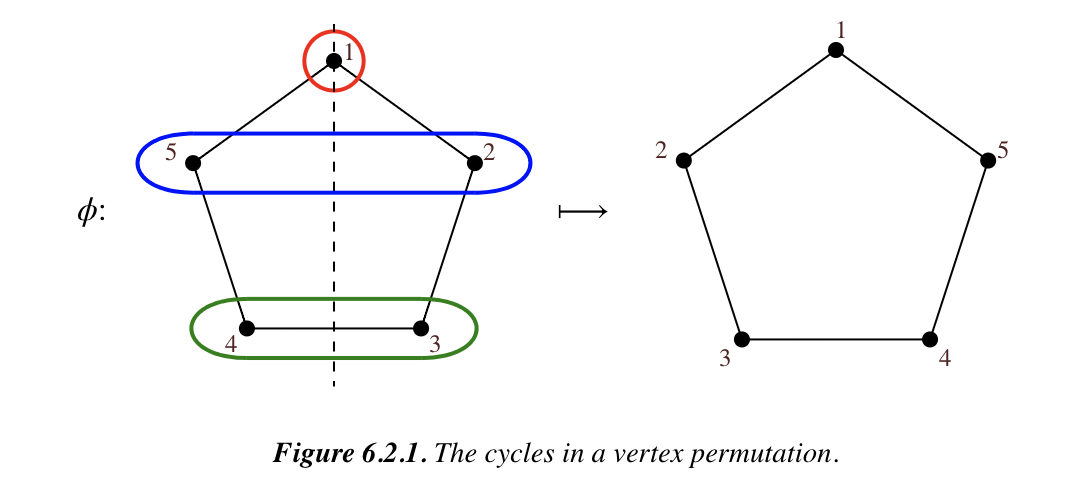
\includegraphics[scale=.6]{pentagon_permutation}
	\end{center}
	\caption{Pentagon Mirror Symmetries}
\end{figure}
\end{solution}

Now let's consider the rotations. For $\rho$, all vertices must be the same color. Thus, there are $7$ fixed colorings for $\rho$. Actually, for a pentagon, all rotations must consist of a single cycle (except the identity), so there are $7$ fixed colorings for each rotation. The identity permutation fixes everything, so there are $7^5$ possible colorings. Then by Burnside's theorem, the solution is
\begin{equation}
	\frac{1}{10}(7^5 + 4 \times 7 + 5 \times 7^3)
\end{equation}

\begin{exercise}
	Verify by direct calculation that Burnside's formula for the number of orbits holds for the action of $D_4$ on the vertices of a square.
\end{exercise}
\begin{solution}
	By inspection, there is only one orbit. The identity element has $4$ fixed points. Then, the rotations have no fixed points/vertices. The two mirror symmetries that connect a vertex to a vertex each have two fixed points/vertices. The remaining two mirror symmetries (which go from midpoint to midpoint) have no fixed points. Therefore, by Burnside's formula, the number of orbits $N$ of the action of $D_4$ on the vertices of a square is
	\begin{equation}
		\frac{1}{8}(4 + 0 + 0 + 0 + 0 + 2 + 0 + 2) = 1
	\end{equation}
\end{solution}

\begin{exercise}
	Let a group $G$ act on itself by conjugation. Show that the action is faithful if and only if $Z(G) = \{1\}$.
\end{exercise}
\begin{solution}
	$\rightarrow$ Suppose the action is faithful. This means that if $gxg^{-1} = x$ for all $x \in G$, then $g = 1$. Then
	\begin{align*}
		Z(G) &= \{ g \in G | gx = xg \quad \forall x\in G \} \\
		&= \{ g \in G | x = gxg^{-1} \quad \forall x\in G \} \\
		&= \{1 \} \tag{since the action is faithful}
	\end{align*}

	$\leftarrow$ Suppose $Z(G) = \{1\}$. Consider a $g \in G$ such that $gxg^{-1} = x$ for all $x \in G$. This implies $gx = xg$ for all $x \in G$, and that $g \in Z(G)$. Therefore $g = 1$, so that the action is faithful. 
\end{solution}

\begin{exercise}
	Let $G$ be a group such that $G/Z(G)$ is cyclic. Then $G$ is abelian.
\end{exercise}
\begin{solution}
	Since $G/Z(G)$ is cyclic, there exists an $x \in G$ such that $G/Z(G) = \langle x Z(G) \rangle$. Now fix $g \in G$. There must be some $m \in \mathbb{N}$ such that $gZ(G) = (xZ(G))^m = x^m Z(G)$. This implies that $(x^m)^{-1} g \in Z(G)$, so that there must exist some $z \in Z(G)$ such that $(x^m)^{-1} g = z$. This implies $g = x^m z$. Now consider another element $h \in G$. by the same logic, there must exist an $n \in \mathbb{N}$ and $z' \in Z(G)$ such that $h = x^n z'$. Then
	\begin{align*}
	gh &= x^m z x^n z' \\
	&= x^m x^n z z' \tag{since $z \in Z(G)$} \\
	&= x^{m + n} z' z \tag{combine powers and $z' \in Z(G)$} \\
	&= x^{n + m} z' z \\
	&= x^n x^m z' z \\
	&= x^n z' x^m z \\
	&= hg 
	\end{align*}
	Therefore $G$ is abelian. 
\end{solution}

\begin{exercise}
	Let $G$ be a group acting on a set $X$ and let $x,y \in X$. Suppose that for some $g \in G$ we have $gx = y$. Show $gG_xg^{-1} = G_y$.
\end{exercise}
\begin{solution}
	We show two inclusions.
	\begin{enumerate}
		\item $\subseteq$: First let $h \in G_x$. We want to show that $ghg^{-1} \in G_y$, so that $ghg^{-1}(y) = y$.  Then
		\begin{align*}
			ghg^{-1}(y) &= gh(x) \tag{$g(x) = y$ implies $x = g^{-1}y$} \\
			&= g(x) \tag{since $h \in G_x$} \\
			&= y 
		\end{align*}
		Therefore $gG_xg^{-1} \subseteq G_y$.
		\item $\supseteq$: Fix $h \in G_y$. We want to show that $h \in gG_xg^{-1}$, or that there exists some $h' \in G_x$ such that $h = gh'g^{-1}$. Let $h' = g^{-1}hg$, and we'll show $h' \in G_x$. Then
		\begin{align*}
			g^{-1}hg(x) &= g^{-1}h(y) \\
			&= g^{-1}(y) \tag{since $h \in G_y$} \\
			&= x
		\end{align*}
		Thus $h' \in G_x$. This implies that$h = gh'g^{-1} \in gG_xg^{-1}$ so that $gG_xg^{-1} \supseteq G_y$. 
	\end{enumerate}
\end{solution}

\begin{exercise}
	Let $G$ be a group that acts transitively on a set $X$. Show that for every $x,y \in X$, we have $G_x \cong G_y$. 
\end{exercise}
\begin{solution}
	We can apply the above exercise to notice that $G_y = gG_xg^{-1}$, where $g(x) = y$ (this $g$ exists by transitivity). We then define a function $\phi : G_x \to G_y = gG_xg^{-1}$ by $\phi(h) = ghg^{-1}$. We claim that $\phi$ is an isomorphism (that is is a homomorphism which is injective and surjective). 
\end{solution}

\begin{exercise}
Let $G$ be an abelian group that acts transitively and faithfully on a set $X$. Show that the action is free. 
\end{exercise}
\begin{solution}
\end{solution}

\subsection{Homework 8}
\begin{exercise}
	Write explicitly the injective homomorphism from $(\Z/2 \Z) \times (\Z/2 \Z)$ to $S_4$ given by Cayley's theorem. 
\end{exercise}
\begin{solution}
	Motivated by the proof of Cayley's theorem, we should consider the action of $G$ on itself by (left) multiplication. Observe that $(\Z/2 \Z) \times (\Z/2 \Z)$ has 4 elements: $\{(0,0),(0,1),(1,0),(1,1)\}$. Also note that $S_4$ permutes $4$ elements. This motivates labeling the $4$ elements in $(\Z/2 \Z) \times (\Z/2 \Z)$  and using left multiplication to create permutations of elements. For example, call the elements 1, 2, 3, and 4. Then
	\begin{align*}
	&2 + 1 = (0,1) = 2\\
	&2 + 2 = (0,0) = 1\\
	&2 + 3 = (1,1) = 4\\
	&2 + 4 = (1,0) = 3 
	\end{align*}
	And we can view this as the permutation $(12)(43)$.
	\begin{align*}
	&3 + 1 = (1,0) = 3\\
	&3 + 2 = (1,1) = 4\\
	&3 + 3 = (0,0) = 1\\
	&3 + 4 = (0,1) = 2 
	\end{align*}
	And we can view this as the permutation $(13)(42)$.
	\begin{align*}
	&4 + 1 = (1,1) = 4\\
	&4 + 2 = (1,0) = 3\\
	&4 + 3 = (0,1) = 2\\
	&4 + 4 = (0,0) = 1 
	\end{align*}
	And we can view this as the permutation $(14)(32)$. Finally applying $(0,0)$ results in the identity permutation. 
 \end{solution}

 \begin{exercise}
 	Show that the group $(\Z / 11 \Z)^{\times}$ is cyclic.
 \end{exercise}
 \begin{solution}
 	Observe that the element $2$ generates $(\Z / 11 \Z)^{\times}$.
 \end{solution}

 \begin{exercise}
	 Show that the group $(\Z / 8 \Z)^{\times}$ is not cyclic.
 \end{exercise}
 \begin{solution}
 	Recall that $(\Z / 8 \Z)^{\times} = \{1,3,5,7\}$. Therefore $|(\Z / 8 \Z)^{\times}| = 4$. We'll demonstrate two subgroups of order $2$, which shows that the group cannot be cyclic. Consider $\{1,3\}$ and $\{1,5\}$. Both of these are (cyclic) subgroups of order $2$, which means that $(\Z / 8 \Z)^{\times}$ cannot be cyclic, since for each $m$ which divides the order of $(\Z / 8 \Z)^{\times}$, we must have a unique subgroup of order $m$. 
 \end{solution}

 \begin{exercise}
 	Find the inverse of each element in $(\Z / 13 \Z)^{\times}$. 
 \end{exercise}
 \begin{solution}
 	Make multiplication table. 
 \end{solution}

\subsection{Homework 9}
\begin{exercise}
Write explicitly the elements of $Z(D_4)$ and of $Z(D_5)$.
\end{exercise}
\begin{solution}
More generally, the center of the Dihedral Group $D_n$ is trivial when $n$ is odd. When $n$ is even, the center consists of the identity element together with the $180$ degree rotation of the polygon.
\end{solution}

\begin{exercise}
	Let $G$ be a group of order 60 that has a normal subgroup of $N$ of order $10$. Show that $G$ has a subgroup of index $2$.
\end{exercise}
\begin{solution} \color{Red}{(Sketchy)}
	\color{Black}
	By Lagrange's theorem,
	\begin{equation}
		\vert G/ N \vert = \frac{|G|}{|N|} = \frac{60}{10} = 6
	\end{equation}
	Then, Cauchy's theorem guarantees the existence of an element $H \leq G/N$ with order $3$ (since 3 divides 6).  Note that $H$ is a subgroup of order $3$. The index of this subgroup in $G$ is then
	\begin{equation}
		[G/N:H] = \frac{|G|}{|N|} \cdot \frac{1}{|H|} = \frac{6}{3} = 2
	\end{equation}
\end{solution}

\begin{exercise}
	Let $G$ be an abelian group of order divisible by 14. Show that $G$ has an element of order 14.
\end{exercise}
\begin{solution}
	By Cauchy's theorem, we know there exists an element $x$ of order 2 and an element $y$ of order 7. We then claim that $xy$ has order 14. This result generalizes. If $G$ is an abelian group, and $x$ and $y$ are elements of $G$ with orders $m$ and $n$ respectively, then if $m$ and $n$ are relatively prime, the order of the element $xy$ is $mn$. We'll prove this more general statement. Note that
	\begin{align*}
	(xy)^{mn} &= x^{mn} y^{mn} \tag{since $G$ is abelian} \\ 
	&= (x^m)^n (y^n)^m \\
	&= 1
	\end{align*}
	Thus the order $r$ of $xy$ divides $mn$. Given that $r$ is the order of $xy$, we also know that 
	\begin{align*}
	1 = (xy)^r = x^r y^r \tag{since $G$ abelian}
	\end{align*}
	Further
	\begin{align*}
	1 = 1^n = x^{rn} y^{rn} = x^{rn} \tag{since $y^n = 1$}.
	\end{align*}
	Thus the order of $x$, $m$, divides $rn$. An analogous argument shows that the order of $y$, $n$, divides $rm$. Thus we get that $mn$ divides $r$ since $m$ and $n$ are relatively prime. Therefore $r = mn$, so that the order of $xy$ is $mn$. 

	In the context of this problem, since $2$ and $7$ are relatively prime, we know that the order of $xy$ is 14.
\end{solution}

\begin{exercise}
Write explicitly the conjugacy classes of $D_6$ and $D_7$. 
\end{exercise}
\begin{solution}
More generally, we can calculate the conjugacy classes of $D_n$ as follows. The identity element always forms its own conjugacy class $\{1\}$. Consider a rotation $\rho^k$. First conjugate by another rotation $\rho^m$:
\begin{align*}
	\rho^m \rho^k \rho^{-m} &= \rho^k
\end{align*}	
Next conjugate by a reflection $\e \rho^m$:
\begin{align*}
	\e \rho^m \rho^k (\e \rho^m)^{-1} &= \e \rho^m \rho^k \rho^{-m} \e^{-1} \\
	&= \e \rho^m \rho^k \rho^{-m} \e \\
	&= \e \rho^k \e \\
	&= \e \e \rho^{-k} \\
	&= \rho^{-k}
\end{align*}
Thus, if $n$ is odd, there will be $\frac{n-1}{2}$ conjugacy classes of size $2$ that contain a rotation and its inverse rotation (i.e.\ $\{\rho^{\pm i}\}$). If $n$ is even, there will be $\frac{n}{2}-1$ conjugacy classes of size $2$ that contain a rotation and its inverse rotation.  

Consider the reflection $\e$. First conjugate by the rotation $\rho^m$:
\begin{align*}
	\rho^m \e \rho^{-m} &= \rho^m \rho^m \e \\
	&= \rho^{2m} \e \\
	&= \e \rho^{-2m} 
\end{align*}
Next conjugate by another reflection $\e\rho^m$:
\begin{align*}
	\e \rho^m \e (\e \rho^m)^{-1} &= \e \rho^m \e \rho^{-m} \e^{-1} \\
	&= \e \rho^m \e \rho^{-m} \e \\
	&= \e \rho^m \rho^{m} \e \e \\
	&= \e \rho^{2m}
\end{align*}
Thus, if $n$ is odd, the reflections all fall in the same conjugacy class. If $n$ is even, the reflections will fall into two conjugacy classes: the reflections where the rotation is an even power and the reflections where the rotation is an odd power. 

For the specific cases requested:
\begin{align*}
	&D_6: \quad \{1\}, \{\rho, \rho^5\}, \{\rho^2, \rho^4\}, \{\rho^3\}, \{\e,\e\rho^2, \e\rho^4\}, \{\e\rho, \e\rho^3, \e\rho^5\} \\
	&D_7: \quad \{1\}, \{\rho, \rho^6\}, \{\rho^2,\rho^5\}, \{\rho^3,\rho^4\}, \{\e, \e\rho, \ldots, \e\rho^6\}
\end{align*}
\end{solution}

\subsection{Homework 10}

\subsection{Homework 11}
\begin{exercise}
	Let $A$ be a commutative ring. We say that $a \in A$ is invertible if there exists some $b \in A$ such that $ab = 1$. Denote by $A^{\times}$ the subset of invertible elements in $A$. 
	\begin{enumerate}
		\item Show that $A^{\times}$ is abelian group.
		\item Show that $A$ is a field if and only if $A^{\times} = A \{0\}$.
		\item Show that $\R[X]^{\times} = \R^{\times}$.
	\end{enumerate}
\end{exercise}
\begin{solution}
We prove each statement as follows:
\begin{enumerate}
	\item Trivial.
	\item Also trivial.
	\item Any non-degenerate polynomial does not have an inverse that is also a polynomial.
\end{enumerate}
\end{solution}

\begin{exercise}
	Let $S$ be a set, and let $P(S)$ be the collection of all subset of $S$. Show that $P(S)$ is a commutative ring with respect to the binary operations of symmetric difference and intersection. 
\end{exercise}

\section{Honors Questions}
\begin{exercise}
From homework 1, we showed that if $g^2 = 1$ for all $g \in G$ where $G$ is a group, then $G$ is abelian. Note that $ab = ba$ iff $aba^{-1}b^{-1} = 1$. Can we write $aba^{-1}b^{-1}$ as a product of squares $c_1 c_2 c_3 \ldots $? (And then each $c^2_i = 1$).
\end{exercise}
\begin{solution}

\end{solution}


\end{document}